% Options for packages loaded elsewhere
\PassOptionsToPackage{unicode}{hyperref}
\PassOptionsToPackage{hyphens}{url}
%
\documentclass[
]{article}
\title{Guide on reproducing Change-by-state graphic}
\author{Xianbin Xu}
\date{8/24/2022}

\usepackage{amsmath,amssymb}
\usepackage{lmodern}
\usepackage{iftex}
\ifPDFTeX
  \usepackage[T1]{fontenc}
  \usepackage[utf8]{inputenc}
  \usepackage{textcomp} % provide euro and other symbols
\else % if luatex or xetex
  \usepackage{unicode-math}
  \defaultfontfeatures{Scale=MatchLowercase}
  \defaultfontfeatures[\rmfamily]{Ligatures=TeX,Scale=1}
\fi
% Use upquote if available, for straight quotes in verbatim environments
\IfFileExists{upquote.sty}{\usepackage{upquote}}{}
\IfFileExists{microtype.sty}{% use microtype if available
  \usepackage[]{microtype}
  \UseMicrotypeSet[protrusion]{basicmath} % disable protrusion for tt fonts
}{}
\makeatletter
\@ifundefined{KOMAClassName}{% if non-KOMA class
  \IfFileExists{parskip.sty}{%
    \usepackage{parskip}
  }{% else
    \setlength{\parindent}{0pt}
    \setlength{\parskip}{6pt plus 2pt minus 1pt}}
}{% if KOMA class
  \KOMAoptions{parskip=half}}
\makeatother
\usepackage{xcolor}
\IfFileExists{xurl.sty}{\usepackage{xurl}}{} % add URL line breaks if available
\IfFileExists{bookmark.sty}{\usepackage{bookmark}}{\usepackage{hyperref}}
\hypersetup{
  pdftitle={Guide on reproducing Change-by-state graphic},
  pdfauthor={Xianbin Xu},
  hidelinks,
  pdfcreator={LaTeX via pandoc}}
\urlstyle{same} % disable monospaced font for URLs
\usepackage[margin=1in]{geometry}
\usepackage{color}
\usepackage{fancyvrb}
\newcommand{\VerbBar}{|}
\newcommand{\VERB}{\Verb[commandchars=\\\{\}]}
\DefineVerbatimEnvironment{Highlighting}{Verbatim}{commandchars=\\\{\}}
% Add ',fontsize=\small' for more characters per line
\usepackage{framed}
\definecolor{shadecolor}{RGB}{248,248,248}
\newenvironment{Shaded}{\begin{snugshade}}{\end{snugshade}}
\newcommand{\AlertTok}[1]{\textcolor[rgb]{0.94,0.16,0.16}{#1}}
\newcommand{\AnnotationTok}[1]{\textcolor[rgb]{0.56,0.35,0.01}{\textbf{\textit{#1}}}}
\newcommand{\AttributeTok}[1]{\textcolor[rgb]{0.77,0.63,0.00}{#1}}
\newcommand{\BaseNTok}[1]{\textcolor[rgb]{0.00,0.00,0.81}{#1}}
\newcommand{\BuiltInTok}[1]{#1}
\newcommand{\CharTok}[1]{\textcolor[rgb]{0.31,0.60,0.02}{#1}}
\newcommand{\CommentTok}[1]{\textcolor[rgb]{0.56,0.35,0.01}{\textit{#1}}}
\newcommand{\CommentVarTok}[1]{\textcolor[rgb]{0.56,0.35,0.01}{\textbf{\textit{#1}}}}
\newcommand{\ConstantTok}[1]{\textcolor[rgb]{0.00,0.00,0.00}{#1}}
\newcommand{\ControlFlowTok}[1]{\textcolor[rgb]{0.13,0.29,0.53}{\textbf{#1}}}
\newcommand{\DataTypeTok}[1]{\textcolor[rgb]{0.13,0.29,0.53}{#1}}
\newcommand{\DecValTok}[1]{\textcolor[rgb]{0.00,0.00,0.81}{#1}}
\newcommand{\DocumentationTok}[1]{\textcolor[rgb]{0.56,0.35,0.01}{\textbf{\textit{#1}}}}
\newcommand{\ErrorTok}[1]{\textcolor[rgb]{0.64,0.00,0.00}{\textbf{#1}}}
\newcommand{\ExtensionTok}[1]{#1}
\newcommand{\FloatTok}[1]{\textcolor[rgb]{0.00,0.00,0.81}{#1}}
\newcommand{\FunctionTok}[1]{\textcolor[rgb]{0.00,0.00,0.00}{#1}}
\newcommand{\ImportTok}[1]{#1}
\newcommand{\InformationTok}[1]{\textcolor[rgb]{0.56,0.35,0.01}{\textbf{\textit{#1}}}}
\newcommand{\KeywordTok}[1]{\textcolor[rgb]{0.13,0.29,0.53}{\textbf{#1}}}
\newcommand{\NormalTok}[1]{#1}
\newcommand{\OperatorTok}[1]{\textcolor[rgb]{0.81,0.36,0.00}{\textbf{#1}}}
\newcommand{\OtherTok}[1]{\textcolor[rgb]{0.56,0.35,0.01}{#1}}
\newcommand{\PreprocessorTok}[1]{\textcolor[rgb]{0.56,0.35,0.01}{\textit{#1}}}
\newcommand{\RegionMarkerTok}[1]{#1}
\newcommand{\SpecialCharTok}[1]{\textcolor[rgb]{0.00,0.00,0.00}{#1}}
\newcommand{\SpecialStringTok}[1]{\textcolor[rgb]{0.31,0.60,0.02}{#1}}
\newcommand{\StringTok}[1]{\textcolor[rgb]{0.31,0.60,0.02}{#1}}
\newcommand{\VariableTok}[1]{\textcolor[rgb]{0.00,0.00,0.00}{#1}}
\newcommand{\VerbatimStringTok}[1]{\textcolor[rgb]{0.31,0.60,0.02}{#1}}
\newcommand{\WarningTok}[1]{\textcolor[rgb]{0.56,0.35,0.01}{\textbf{\textit{#1}}}}
\usepackage{graphicx}
\makeatletter
\def\maxwidth{\ifdim\Gin@nat@width>\linewidth\linewidth\else\Gin@nat@width\fi}
\def\maxheight{\ifdim\Gin@nat@height>\textheight\textheight\else\Gin@nat@height\fi}
\makeatother
% Scale images if necessary, so that they will not overflow the page
% margins by default, and it is still possible to overwrite the defaults
% using explicit options in \includegraphics[width, height, ...]{}
\setkeys{Gin}{width=\maxwidth,height=\maxheight,keepaspectratio}
% Set default figure placement to htbp
\makeatletter
\def\fps@figure{htbp}
\makeatother
\setlength{\emergencystretch}{3em} % prevent overfull lines
\providecommand{\tightlist}{%
  \setlength{\itemsep}{0pt}\setlength{\parskip}{0pt}}
\setcounter{secnumdepth}{-\maxdimen} % remove section numbering
\usepackage{amsmath}
\ifLuaTeX
  \usepackage{selnolig}  % disable illegal ligatures
\fi

\begin{document}
\maketitle

\hypertarget{introduction}{%
\subsection{Introduction}\label{introduction}}

This markdown file presents the ways to replicate change-by-state
function, which shows how one variable changed over years for each
state. The function were available for both BRFSS (Behavioral Risk
Factor Surveillance System) and BLS (Bureau of Labor Statistics) data.

This RMD (R Markdown) file had been knitted into a PDF file for easier
reading. PDF file and R Markdown file(end with .rmd) are all included in
the directory under the same name. To reproduce the code, open the R
Markdown in RStudio, then run the whole markdown file.

To get a LaTeX file of the document, add ``keep\_tex: true'' below the
pdf\_output: line, in the header section of R Markdown. Then, knit the
whole markdown file.

Make sure the file is located in \(/\)Graphic\_Reproduction\_Folder,
with directory BRFSS\_Data in the same directory containing
\(/\)Graphic\_Reproduction\_Folder.

Make sure the following files are in place at BRFSS\_Data folder:

\begin{quote}
\begin{quote}
Processed\_BRFSS\_1999\_to\_2020.csv. This can be gained by running
BRFSS\_Fractured\_Download\_Process.R under Default parameters.
\end{quote}
\end{quote}

\begin{quote}
\begin{quote}
Wages\_By\_State.csv and Employement\_By\_State.csv. This can be gained
by running BLS\_Download\_State\_Level.R in BLS\_Data and copy to BRFSS
folder.
\end{quote}
\end{quote}

To use processed BRFSS Data of a different year range, change the
parameter at the head of BRFSS\_Fractured\_Download\_Process.R. See
comment of that script for specific parameters to be used.

The following packages are used:

\begin{Shaded}
\begin{Highlighting}[]
\FunctionTok{library}\NormalTok{(}\StringTok{"readxl"}\NormalTok{) }\DocumentationTok{\#\# To read Excel}
\FunctionTok{library}\NormalTok{(}\StringTok{"dplyr"}\NormalTok{) }\DocumentationTok{\#\# For better data processing}
\FunctionTok{library}\NormalTok{(}\StringTok{"haven"}\NormalTok{) }\DocumentationTok{\#\# To read and export DTA Files}
\FunctionTok{library}\NormalTok{(tidyr) }\DocumentationTok{\#\# Tidy functions}
\FunctionTok{library}\NormalTok{(cdlTools) }\DocumentationTok{\#\# To corresponde FIPS code to state names/abbreviations}
\FunctionTok{library}\NormalTok{(ggplot2) }\DocumentationTok{\#\# To have easier time plotting in R}
\FunctionTok{library}\NormalTok{(gridExtra) }\DocumentationTok{\#\# To place two plots by each other}
\end{Highlighting}
\end{Shaded}

use install.packages() to install if you haven't installed already.

And read the file:

\begin{Shaded}
\begin{Highlighting}[]
\NormalTok{Data }\OtherTok{=} \FunctionTok{read.csv}\NormalTok{(}\AttributeTok{file =} \StringTok{"./../BRFSS\_Data/Processed\_BRFSS\_1999\_to\_2020.csv"}\NormalTok{, }
                \AttributeTok{stringsAsFactors =} \ConstantTok{FALSE}\NormalTok{)}

\CommentTok{\# Specifics: In this dataset, only the specific subdivision of occupations, such as dentist, general, family practitioners, were recorded}
\NormalTok{BLS\_Data\_Specifics }\OtherTok{=} \FunctionTok{read.csv}\NormalTok{(}\AttributeTok{file =} \StringTok{"./../BRFSS\_Data/Wages\_By\_State.csv"}\NormalTok{, }
                              \AttributeTok{stringsAsFactors =} \ConstantTok{FALSE}\NormalTok{)}

\CommentTok{\# General: In this dataset, general division of occupations, such as dentist, all, and physicians and surgeons, all, were recorded as well.}
\NormalTok{BLS\_Data\_General }\OtherTok{=} \FunctionTok{read.csv}\NormalTok{(}\AttributeTok{file =} \StringTok{"./../BRFSS\_Data/Employment\_By\_State.csv"}\NormalTok{, }
                            \AttributeTok{stringsAsFactors =} \ConstantTok{FALSE}\NormalTok{)}
\end{Highlighting}
\end{Shaded}

The Data should be individual entries accumulated over time, each entry
representing a respondent. It have to be processed before using later
on.

\hypertarget{example-graphic-one}{%
\subsection{Example Graphic One}\label{example-graphic-one}}

The graphic here is of same format of the ones we are creating here
today. It is placed for you to have a general idea on the kind of
graphic we are using.

\begin{figure}
\centering
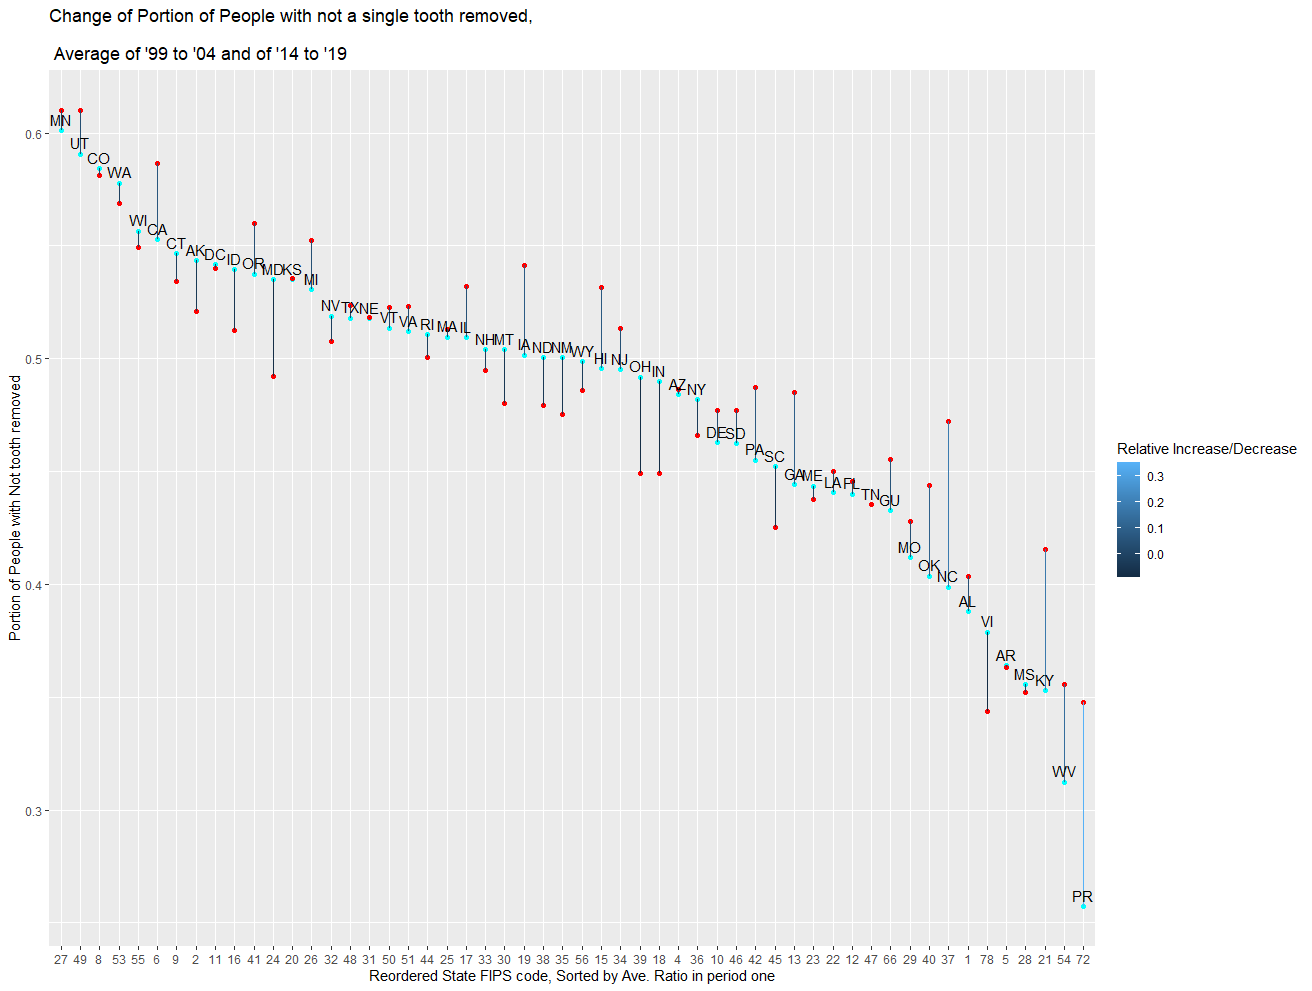
\includegraphics{Change_By_State_01.png}
\caption{Example Graphic One}
\end{figure}

The Graphic shows the change of the portion of people who have not had a
single teeth removed. The cyan dots represents the average of such
ratio, of each state, over year 1999 to year 2004. The red dot are same
variable, but over year 2014 and 2019. The lines connecting two dot
represents the change of the same state over year, while its color,
referring to the scale at the right side, refers to the percentage of
changes.

\hypertarget{processing-data-for-bls}{%
\subsection{Processing Data, for BLS}\label{processing-data-for-bls}}

Since not much of this kind of graphic were asked, I didn't use a
function to trim the data to be used for plotting. Instead, I put in
extensive instructions on where to replace and change if you want to
plot other data.

It is also because that switching between variable names, which must be
edited as character then used in formula, imposed difficulty. Meanwhile
difference in variables also imposed problem.

The one variable would be separated and averaged for two periods of
time, as two variables, which would then be plotted with changes in each
state. The following function is a processor that takes a dataframe and
trim it to what we need for plotting. The resulting dataset would have
two useful columns consisting one variable in input data frame, averaged
or summed over two periods of time. It could thus be used to reflect
changes over time.

Required Input:

\begin{quote}
\begin{quote}
Input\_Data: A data frame with year-state accuracy.
\end{quote}
\end{quote}

\begin{quote}
\begin{quote}
Var\_Name: A character, the name of the variable that is to be processed
(and thus plotted later on)
\end{quote}
\end{quote}

\begin{quote}
\begin{quote}
Year\_Var\_Name: Character, the name of the variable indicating the year
of entry. For BLS, it is ``year''. For BRFSS, it is ``YEAR\_RESPONSE''
\end{quote}
\end{quote}

\begin{quote}
\begin{quote}
State\_Var\_Name: Character, the name of the variable indicating the
state of the entry. For BLS, it is ``st'', which is abbreviation of
states' name. For BRFSS, either ``State'' (full name of states) or
``STATE\_FIPS\_CODE'' (FIPS code of states) shall work.
\end{quote}
\end{quote}

\begin{quote}
\begin{quote}
Sum\_or\_Average: For two year periods, shall the result do sum or
average? Only two options, ``Sum'' and ``Average'' are available, and
default ``Average''.
\end{quote}
\end{quote}

\begin{quote}
\begin{quote}
first\_period: first year period to be used. As a two-element numeric
vector, with default c(1999, 2004)
\end{quote}
\end{quote}

\begin{quote}
\begin{quote}
first\_period: second year period to be used. As a two-element numeric
vector, with default c(2014, 2019)
\end{quote}
\end{quote}

Technical details are below in comments

\begin{Shaded}
\begin{Highlighting}[]
\NormalTok{By\_Year\_Operation }\OtherTok{=} \ControlFlowTok{function}\NormalTok{(Input\_Data, Var\_Name, }
\NormalTok{         Year\_Var\_Name, }
\NormalTok{         State\_Var\_Name, }\AttributeTok{Sum\_or\_Average =} \StringTok{"Average"}\NormalTok{,}
         \AttributeTok{first\_period =} \FunctionTok{c}\NormalTok{(}\DecValTok{1999}\NormalTok{, }\DecValTok{2004}\NormalTok{), }
         \AttributeTok{second\_period =} \FunctionTok{c}\NormalTok{(}\DecValTok{2014}\NormalTok{, }\DecValTok{2019}\NormalTok{))\{}
  
\NormalTok{  temp1 }\OtherTok{=}\NormalTok{ Input\_Data }\SpecialCharTok{\%\textgreater{}\%}
    \FunctionTok{filter}\NormalTok{(}\FunctionTok{get}\NormalTok{(Year\_Var\_Name) }\SpecialCharTok{\textgreater{}=}\NormalTok{ first\_period[}\DecValTok{1}\NormalTok{] }\SpecialCharTok{\&} 
             \FunctionTok{get}\NormalTok{(Year\_Var\_Name) }\SpecialCharTok{\textless{}=}\NormalTok{ first\_period[}\DecValTok{2}\NormalTok{])}
  
\NormalTok{  temp2 }\OtherTok{=}\NormalTok{ Input\_Data }\SpecialCharTok{\%\textgreater{}\%}
    \FunctionTok{filter}\NormalTok{(}\FunctionTok{get}\NormalTok{(Year\_Var\_Name) }\SpecialCharTok{\textgreater{}=}\NormalTok{ second\_period[}\DecValTok{1}\NormalTok{] }\SpecialCharTok{\&} 
             \FunctionTok{get}\NormalTok{(Year\_Var\_Name) }\SpecialCharTok{\textless{}=}\NormalTok{ second\_period[}\DecValTok{2}\NormalTok{])}
  \DocumentationTok{\#\#\# Filter the data into two parts,}
  \DocumentationTok{\#\#\# Each only taking from the year designated by }
  \DocumentationTok{\#\#\# first\_period and second\_period}
  
  \ControlFlowTok{if}\NormalTok{(Sum\_or\_Average }\SpecialCharTok{==} \StringTok{"Average"}\NormalTok{)\{}
\NormalTok{    Var\_Name\_1 }\OtherTok{=} \FunctionTok{paste}\NormalTok{(Var\_Name, }\StringTok{"\_Average\_"}\NormalTok{,}
\NormalTok{                             first\_period[}\DecValTok{1}\NormalTok{], }\StringTok{"\_"}\NormalTok{, first\_period[}\DecValTok{2}\NormalTok{],}
                             \AttributeTok{sep =} \StringTok{""}\NormalTok{)}
    \DocumentationTok{\#\#\# Designate variable names for the first period.}
    \DocumentationTok{\#\#\# Format: Original\_Var\_Name\_Average\_begin\_year\_end\_year.}
    
\NormalTok{    Var\_Name\_2 }\OtherTok{=} \FunctionTok{paste}\NormalTok{(Var\_Name, }\StringTok{"\_Average\_"}\NormalTok{,}
\NormalTok{                             second\_period[}\DecValTok{1}\NormalTok{], }\StringTok{"\_"}\NormalTok{, second\_period[}\DecValTok{2}\NormalTok{],}
                             \AttributeTok{sep =} \StringTok{""}\NormalTok{)}
    
\NormalTok{    temp1 }\OtherTok{=}\NormalTok{ temp1 }\SpecialCharTok{\%\textgreater{}\%} 
      \FunctionTok{group\_by\_at}\NormalTok{(State\_Var\_Name) }\SpecialCharTok{\%\textgreater{}\%}
      \FunctionTok{summarise\_at}\NormalTok{(Var\_Name, mean, }\AttributeTok{na.rm =} \ConstantTok{TRUE}\NormalTok{) }\SpecialCharTok{\%\textgreater{}\%}
      \FunctionTok{rename\_at}\NormalTok{(Var\_Name, }
                \SpecialCharTok{\textasciitilde{}}\NormalTok{Var\_Name\_1)}
    
    \DocumentationTok{\#\#\# For each state, find the mean of the variable}
    \DocumentationTok{\#\#\# Designated by input Var\_Name. This dataset,}
    \DocumentationTok{\#\#\# the temp1, shall consist only entries from the first period,}
    \DocumentationTok{\#\#\# Thus directly summarising would be of no problem.}
    \DocumentationTok{\#\#\# The variable would be renamed for later use.}
    
\NormalTok{    temp2 }\OtherTok{=}\NormalTok{ temp2 }\SpecialCharTok{\%\textgreater{}\%} 
      \FunctionTok{group\_by\_at}\NormalTok{(State\_Var\_Name) }\SpecialCharTok{\%\textgreater{}\%}
      \FunctionTok{summarise\_at}\NormalTok{(Var\_Name, mean, }\AttributeTok{na.rm =} \ConstantTok{TRUE}\NormalTok{) }\SpecialCharTok{\%\textgreater{}\%}
      \FunctionTok{rename\_at}\NormalTok{(Var\_Name, }
                \SpecialCharTok{\textasciitilde{}}\NormalTok{Var\_Name\_2)}
    
    \DocumentationTok{\#\#\# Same for second part (for second period)}

\NormalTok{  \}}\ControlFlowTok{else} \ControlFlowTok{if}\NormalTok{(Sum\_or\_Average }\SpecialCharTok{==} \StringTok{"Sum"}\NormalTok{)\{}
\NormalTok{    Var\_Name\_1 }\OtherTok{=} \FunctionTok{paste}\NormalTok{(Var\_Name, }\StringTok{"\_Sum\_"}\NormalTok{,}
\NormalTok{                             first\_period[}\DecValTok{1}\NormalTok{], }\StringTok{"\_"}\NormalTok{, first\_period[}\DecValTok{2}\NormalTok{],}
                             \AttributeTok{sep =} \StringTok{""}\NormalTok{)}
    
\NormalTok{    Var\_Name\_2 }\OtherTok{=} \FunctionTok{paste}\NormalTok{(Var\_Name, }\StringTok{"\_Sum\_"}\NormalTok{,}
\NormalTok{                             second\_period[}\DecValTok{1}\NormalTok{], }\StringTok{"\_"}\NormalTok{, second\_period[}\DecValTok{2}\NormalTok{],}
                             \AttributeTok{sep =} \StringTok{""}\NormalTok{)}
    
\NormalTok{    temp1 }\OtherTok{=}\NormalTok{ temp1 }\SpecialCharTok{\%\textgreater{}\%} 
      \FunctionTok{group\_by\_at}\NormalTok{(State\_Var\_Name) }\SpecialCharTok{\%\textgreater{}\%}
      \FunctionTok{summarise\_at}\NormalTok{(Var\_Name, sum, }\AttributeTok{na.rm =} \ConstantTok{TRUE}\NormalTok{) }\SpecialCharTok{\%\textgreater{}\%}
      \FunctionTok{rename\_at}\NormalTok{(Var\_Name, }
                \SpecialCharTok{\textasciitilde{}}\NormalTok{Var\_Name\_1)}
    
\NormalTok{    temp2 }\OtherTok{=}\NormalTok{ temp2 }\SpecialCharTok{\%\textgreater{}\%} 
      \FunctionTok{group\_by\_at}\NormalTok{(State\_Var\_Name) }\SpecialCharTok{\%\textgreater{}\%}
      \FunctionTok{summarise\_at}\NormalTok{(Var\_Name, sum, }\AttributeTok{na.rm =} \ConstantTok{TRUE}\NormalTok{) }\SpecialCharTok{\%\textgreater{}\%}
      \FunctionTok{rename\_at}\NormalTok{(Var\_Name, }
                \SpecialCharTok{\textasciitilde{}}\NormalTok{Var\_Name\_2)}
    
    \DocumentationTok{\#\#\# Doing the same thing except changing Average to Sum}
\NormalTok{  \}}
  
\NormalTok{  temp }\OtherTok{=} \FunctionTok{left\_join}\NormalTok{(temp1, temp2, }\AttributeTok{by =}\NormalTok{ State\_Var\_Name)}
  \DocumentationTok{\#\# Merge the dataset, by State\_Var\_Name, the name }
  \DocumentationTok{\#\# for the variable which shows which state the entry represents.}
  
\NormalTok{  temp }\OtherTok{=} \FunctionTok{as.data.frame}\NormalTok{(temp)}
  
\NormalTok{  temp}\SpecialCharTok{$}\NormalTok{Diff\_Ratio }\OtherTok{=}\NormalTok{ (temp[, Var\_Name\_2] }\SpecialCharTok{{-}}\NormalTok{ temp[, Var\_Name\_1]) }\SpecialCharTok{/}
\NormalTok{    temp[, Var\_Name\_1]}
  \DocumentationTok{\#\#\# Find the relative difference.}
  \DocumentationTok{\#\#\# Formula: (Result of second period {-} Result first period)/Res. 2nd period}
  
  
\NormalTok{  temp}\SpecialCharTok{$}\NormalTok{State\_FIPS\_Code }\OtherTok{=} \FunctionTok{fips}\NormalTok{(temp[, State\_Var\_Name], }\AttributeTok{to =} \StringTok{"fips"}\NormalTok{)}
  \DocumentationTok{\#\#\# Convert whatever state\_var you used into FIPS code, for easier plotting.}
  
  
  \FunctionTok{return}\NormalTok{(temp)}
  
\NormalTok{         \}}
\end{Highlighting}
\end{Shaded}

\hypertarget{process-the-brfss-data}{%
\subsection{Process the BRFSS Data}\label{process-the-brfss-data}}

Upon plotting the BRFSS Data, we need it to be in State-Year format not
unlike the BLS Data. As such, the same function used for BRFSS data in
BRFSS\_Graphic\_Reproduction.RMD were simply copied here, and please
refer to it for more specific information. Still, all technical comments
were kept here. Namely, the Data\_Condensor function takes a BRFSS
dataset, raw, and a few parameters. It will give out state-year data on
one or two variables.

\begin{Shaded}
\begin{Highlighting}[]
\DocumentationTok{\#\# This is actually the same as another script}

\NormalTok{Data\_Range\_Checker }\OtherTok{=} \ControlFlowTok{function}\NormalTok{(Input\_Data, Var)\{}
\NormalTok{  temp }\OtherTok{=}\NormalTok{ Input\_Data }\SpecialCharTok{\%\textgreater{}\%} \FunctionTok{group\_by}\NormalTok{(STATE\_FIPS\_CODE, YEAR\_RESPONSE) }\SpecialCharTok{\%\textgreater{}\%}
    \FunctionTok{summarize}\NormalTok{(}\AttributeTok{Temp1 =} \FunctionTok{across}\NormalTok{(\{\{ Var \}\}, sum, }\AttributeTok{na.rm =} \ConstantTok{TRUE}\NormalTok{)) }\SpecialCharTok{\%\textgreater{}\%}
    \FunctionTok{mutate}\NormalTok{(}\AttributeTok{Temp1 =} \FunctionTok{as.numeric}\NormalTok{(}\FunctionTok{unlist}\NormalTok{(Temp1)))}
\NormalTok{  temp }\OtherTok{=}\NormalTok{ temp[temp}\SpecialCharTok{$}\NormalTok{Temp1 }\SpecialCharTok{\textgreater{}} \DecValTok{0}\NormalTok{, ]}
  \FunctionTok{return}\NormalTok{(temp[, }\DecValTok{1}\SpecialCharTok{:}\DecValTok{2}\NormalTok{])}
\NormalTok{\}}

\NormalTok{Data\_Condensor }\OtherTok{=} \ControlFlowTok{function}\NormalTok{(Input\_Data, Var1, }\AttributeTok{Var2 =} \ConstantTok{NA}\NormalTok{,}
\NormalTok{                          Var1\_Condition, }\AttributeTok{Var1\_Denominator\_Values =} \ConstantTok{NA}\NormalTok{,}
                          \AttributeTok{Var2\_Condition =} \ConstantTok{NA}\NormalTok{, }\AttributeTok{Var2\_Denominator\_Values =} \ConstantTok{NA}\NormalTok{,}
                          \AttributeTok{Num\_or\_Ratio =} \StringTok{"Ratio"}\NormalTok{, }\AttributeTok{Rename\_Columns =} \ConstantTok{FALSE}\NormalTok{,}
                          \AttributeTok{year\_begin =} \DecValTok{1999}\NormalTok{, }\AttributeTok{year\_end =} \DecValTok{2020}\NormalTok{)\{}
  
  
\NormalTok{  temp }\OtherTok{=}\NormalTok{ Input\_Data }\SpecialCharTok{\%\textgreater{}\%}
    \FunctionTok{filter}\NormalTok{(YEAR\_RESPONSE }\SpecialCharTok{\textgreater{}=}\NormalTok{ year\_begin }\SpecialCharTok{\&}\NormalTok{ YEAR\_RESPONSE }\SpecialCharTok{\textless{}=}\NormalTok{ year\_end)}
  \DocumentationTok{\#\#\# Filter the data with year range}
  
\NormalTok{  year\_List\_1 }\OtherTok{=} \FunctionTok{Data\_Range\_Checker}\NormalTok{(temp, Var1)}
  \DocumentationTok{\#\#\# This year\_list\_1 tells us which state{-}year these data would be available}
  
  \ControlFlowTok{if}\NormalTok{(}\SpecialCharTok{!}\FunctionTok{is.na}\NormalTok{(Var2))\{}
    \DocumentationTok{\#\#\# If var2 is not NA, meaning that there is an entry, also check the range}
    \DocumentationTok{\#\#\# for var2.}
\NormalTok{    year\_List\_2 }\OtherTok{=} \FunctionTok{Data\_Range\_Checker}\NormalTok{(temp, Var2)}
    
    \DocumentationTok{\#\#\# Left{-}Join it with year range for Var1. }
    \DocumentationTok{\#\#\# Keeps only common elements, so that year{-}state left here is available}
    \DocumentationTok{\#\#\# All the year.}
\NormalTok{    year\_state\_List }\OtherTok{=} \FunctionTok{inner\_join}\NormalTok{(year\_List\_1, year\_List\_2)}
    
\NormalTok{  \}}\ControlFlowTok{else}\NormalTok{\{}
\NormalTok{    year\_state\_List }\OtherTok{=}\NormalTok{ year\_List\_1}
\NormalTok{  \}}
  
\NormalTok{  temp }\OtherTok{=} \FunctionTok{inner\_join}\NormalTok{(temp, year\_state\_List)}
  \DocumentationTok{\#\#\#Keer only state{-}year that have got available data}
  
  \ControlFlowTok{if}\NormalTok{(}\ConstantTok{TRUE} \SpecialCharTok{\%in\%} \FunctionTok{is.na}\NormalTok{(Var1\_Denominator\_Values))\{}
    \CommentTok{\# No entry is for Var1\_Denominator\_Values. Use Default Setting.}
    \CommentTok{\# Contain everything that ain\textquotesingle{}t not Don\textquotesingle{}t Know, Unsure, or refused.}
    \CommentTok{\# According to codebook, it shall be 1:9 without 7 and 9.}
\NormalTok{    Var1\_Denominator\_Values }\OtherTok{=} \FunctionTok{c}\NormalTok{(}\DecValTok{1}\SpecialCharTok{:}\DecValTok{6}\NormalTok{, }\DecValTok{8}\NormalTok{)}
\NormalTok{  \}}
  
  \CommentTok{\# Sum up by state{-}year, drop those with too small a sample size.}
\NormalTok{  First\_Var\_Result }\OtherTok{=} \FunctionTok{mutate}\NormalTok{(temp, }
                            \AttributeTok{Var1\_Mask =} \FunctionTok{ifelse}\NormalTok{(temp[, Var1] }\SpecialCharTok{\%in\%}\NormalTok{ Var1\_Condition, }
                                               \DecValTok{1}\NormalTok{, }\DecValTok{0}\NormalTok{)) }\SpecialCharTok{\%\textgreater{}\%} 
    \DocumentationTok{\#\#\# Gives 1 to a temporary variable if the Var1}
    \DocumentationTok{\#\#\# Fits in condition}
    \FunctionTok{mutate}\NormalTok{(temp, }\AttributeTok{Var1\_Denominator\_Count =} 
             \FunctionTok{ifelse}\NormalTok{(temp[, Var1] }\SpecialCharTok{\%in\%}\NormalTok{ Var1\_Denominator\_Values, }\DecValTok{1}\NormalTok{, }\DecValTok{0}\NormalTok{)) }\SpecialCharTok{\%\textgreater{}\%}
    \DocumentationTok{\#\#\# Give 1 to a temporary variable if Var1 fits in}
    \DocumentationTok{\#\#\# Denominator Value.}
    \FunctionTok{group\_by}\NormalTok{(STATE\_FIPS\_CODE, YEAR\_RESPONSE) }\SpecialCharTok{\%\textgreater{}\%} 
    \FunctionTok{summarize}\NormalTok{(}\AttributeTok{Var1\_Fit\_Condition\_Sum =} \FunctionTok{sum}\NormalTok{(Var1\_Mask, }\AttributeTok{na.rm =} \ConstantTok{TRUE}\NormalTok{), }
              \AttributeTok{Var1\_Total =} \FunctionTok{sum}\NormalTok{(Var1\_Denominator\_Count, }\AttributeTok{na.rm =} \ConstantTok{TRUE}\NormalTok{)) }\SpecialCharTok{\%\textgreater{}\%}
    \DocumentationTok{\#\#\# Sum the previous temporary variables by state{-}year }
    \DocumentationTok{\#\#\# And write them in two variables for use later on.}
    \FunctionTok{filter}\NormalTok{(Var1\_Fit\_Condition\_Sum }\SpecialCharTok{\textgreater{}=} \DecValTok{100}\NormalTok{)}
  
  \ControlFlowTok{if}\NormalTok{(}\SpecialCharTok{!}\FunctionTok{is.na}\NormalTok{(Var2))\{}
    \CommentTok{\# Var2 is default NA.}
    \CommentTok{\# If anything was put onto Var2, then this chunk shall run, doing the same thing as above.}
    
    \ControlFlowTok{if}\NormalTok{(}\ConstantTok{TRUE} \SpecialCharTok{\%in\%} \FunctionTok{is.na}\NormalTok{(Var2\_Denominator\_Values))\{}
\NormalTok{      Var2\_Denominator\_Values }\OtherTok{=} \FunctionTok{c}\NormalTok{(}\DecValTok{1}\SpecialCharTok{:}\DecValTok{6}\NormalTok{, }\DecValTok{8}\NormalTok{)}
\NormalTok{    \}}
\NormalTok{    Second\_Var\_Result }\OtherTok{=}\NormalTok{ temp }\SpecialCharTok{\%\textgreater{}\%} 
      \FunctionTok{mutate}\NormalTok{(}\AttributeTok{Var2\_Mask =} \FunctionTok{ifelse}\NormalTok{(temp[, Var2] }\SpecialCharTok{\%in\%}\NormalTok{ Var2\_Condition, }\DecValTok{1}\NormalTok{, }\DecValTok{0}\NormalTok{)) }\SpecialCharTok{\%\textgreater{}\%} 
      \FunctionTok{mutate}\NormalTok{(temp, }\AttributeTok{Var2\_Denominator\_Count =} 
               \FunctionTok{ifelse}\NormalTok{(temp[, Var2] }\SpecialCharTok{\%in\%}\NormalTok{ Var2\_Denominator\_Values, }\DecValTok{1}\NormalTok{, }\DecValTok{0}\NormalTok{)) }\SpecialCharTok{\%\textgreater{}\%}
      \FunctionTok{group\_by}\NormalTok{(STATE\_FIPS\_CODE, YEAR\_RESPONSE) }\SpecialCharTok{\%\textgreater{}\%} 
      \FunctionTok{summarize}\NormalTok{(}\AttributeTok{Var2\_Fit\_Condition\_Sum =} \FunctionTok{sum}\NormalTok{(Var2\_Mask, }\AttributeTok{na.rm =} \ConstantTok{TRUE}\NormalTok{), }
                \AttributeTok{Var2\_Total =} \FunctionTok{sum}\NormalTok{(Var2\_Denominator\_Count, }\AttributeTok{na.rm =} \ConstantTok{TRUE}\NormalTok{)) }\SpecialCharTok{\%\textgreater{}\%}
      \FunctionTok{filter}\NormalTok{(Var2\_Fit\_Condition\_Sum }\SpecialCharTok{\textgreater{}=} \DecValTok{100}\NormalTok{)}
    
    \DocumentationTok{\#\#\# Re{-}write temp dataframe as inner{-}join of the }
    \DocumentationTok{\#\#\# result from calculating two variables}
\NormalTok{    temp }\OtherTok{=} \FunctionTok{inner\_join}\NormalTok{(First\_Var\_Result, Second\_Var\_Result)}
\NormalTok{  \}}\ControlFlowTok{else}\NormalTok{\{}
    \DocumentationTok{\#\#\# No variable 2. Use only variable 1 result.}
\NormalTok{    temp }\OtherTok{=}\NormalTok{ First\_Var\_Result}
\NormalTok{  \}}
  
  
  \ControlFlowTok{if}\NormalTok{(Num\_or\_Ratio }\SpecialCharTok{==} \StringTok{"Ratio"}\NormalTok{)\{}
    \CommentTok{\# Find ratios for var1.}
\NormalTok{    temp }\OtherTok{=}\NormalTok{ temp }\SpecialCharTok{\%\textgreater{}\%} \FunctionTok{mutate}\NormalTok{(}\AttributeTok{Var1\_Ratio =}\NormalTok{ Var1\_Fit\_Condition\_Sum }\SpecialCharTok{/}\NormalTok{ Var1\_Total)}
    \CommentTok{\# rename, if Rename\_Columns was TRUE.}
    \ControlFlowTok{if}\NormalTok{(Rename\_Columns)\{}
\NormalTok{      temp }\OtherTok{=}\NormalTok{ temp }\SpecialCharTok{\%\textgreater{}\%} 
        \FunctionTok{rename\_at}\NormalTok{(}\FunctionTok{vars}\NormalTok{(}\FunctionTok{c}\NormalTok{(}\StringTok{"Var1\_Fit\_Condition\_Sum"}\NormalTok{, }\StringTok{"Var1\_Total"}\NormalTok{, }\StringTok{"Var1\_Ratio"}\NormalTok{)),}
                  \SpecialCharTok{\textasciitilde{}} \FunctionTok{c}\NormalTok{(}\FunctionTok{paste}\NormalTok{(Var1, }\StringTok{"\_Fit\_Condition\_Count"}\NormalTok{, }\AttributeTok{sep =} \StringTok{""}\NormalTok{),}
                      \FunctionTok{paste}\NormalTok{(Var1, }\StringTok{"\_Total"}\NormalTok{, }\AttributeTok{sep =} \StringTok{""}\NormalTok{),}
                      \FunctionTok{paste}\NormalTok{(Var1, }\StringTok{"\_Ratio"}\NormalTok{, }\AttributeTok{sep =} \StringTok{""}\NormalTok{)))}
\NormalTok{    \}}
    \ControlFlowTok{if}\NormalTok{(}\SpecialCharTok{!}\FunctionTok{is.na}\NormalTok{(Var2))\{}
      \CommentTok{\# Do the same thing for Var2, if it was calculated.}
\NormalTok{      temp }\OtherTok{=}\NormalTok{ temp }\SpecialCharTok{\%\textgreater{}\%} 
        \FunctionTok{mutate}\NormalTok{(}\AttributeTok{Var2\_Ratio =}\NormalTok{ Var2\_Fit\_Condition\_Sum }\SpecialCharTok{/}\NormalTok{ Var2\_Total)}
      \ControlFlowTok{if}\NormalTok{(Rename\_Columns)\{}
\NormalTok{        temp }\OtherTok{=}\NormalTok{ temp }\SpecialCharTok{\%\textgreater{}\%} 
          \FunctionTok{rename\_at}\NormalTok{(}\FunctionTok{vars}\NormalTok{(}\FunctionTok{c}\NormalTok{(}\StringTok{"Var2\_Fit\_Condition\_Sum"}\NormalTok{, }
                           \StringTok{"Var2\_Total"}\NormalTok{, }\StringTok{"Var2\_Ratio"}\NormalTok{)),}
                    \SpecialCharTok{\textasciitilde{}} \FunctionTok{c}\NormalTok{(}\FunctionTok{paste}\NormalTok{(Var2, }\StringTok{"\_Fit\_Condition\_Count"}\NormalTok{, }\AttributeTok{sep =} \StringTok{""}\NormalTok{),}
                        \FunctionTok{paste}\NormalTok{(Var2, }\StringTok{"\_Total"}\NormalTok{, }\AttributeTok{sep =} \StringTok{""}\NormalTok{),}
                        \FunctionTok{paste}\NormalTok{(Var2, }\StringTok{"\_Ratio"}\NormalTok{, }\AttributeTok{sep =} \StringTok{""}\NormalTok{)))}
\NormalTok{      \}}
\NormalTok{    \}}
\NormalTok{  \}}
  \ControlFlowTok{else}\NormalTok{\{}
    \DocumentationTok{\#\#\# No Ratio Calculated. Do Rename here.}
    \ControlFlowTok{if}\NormalTok{(Rename\_Columns)\{}
\NormalTok{      temp }\OtherTok{=}\NormalTok{ temp }\SpecialCharTok{\%\textgreater{}\%} 
        \FunctionTok{rename\_at}\NormalTok{(}\FunctionTok{vars}\NormalTok{(}\FunctionTok{c}\NormalTok{(}\StringTok{"Var1\_Fit\_Condition\_Sum"}\NormalTok{, }\StringTok{"Var1\_Total"}\NormalTok{)), }
                  \SpecialCharTok{\textasciitilde{}} \FunctionTok{c}\NormalTok{(}\FunctionTok{paste}\NormalTok{(Var1, }\StringTok{"\_Fit\_Condition\_Count"}\NormalTok{, }\AttributeTok{sep =} \StringTok{""}\NormalTok{),}
                      \FunctionTok{paste}\NormalTok{(Var1, }\StringTok{"\_Total"}\NormalTok{, }\AttributeTok{sep =} \StringTok{""}\NormalTok{)))}
\NormalTok{    \}}
    \ControlFlowTok{if}\NormalTok{(}\SpecialCharTok{!}\FunctionTok{is.na}\NormalTok{(Var2))\{}
\NormalTok{      temp }\OtherTok{=}\NormalTok{ temp }\SpecialCharTok{\%\textgreater{}\%} \FunctionTok{mutate}\NormalTok{(}\AttributeTok{Var2\_Ratio =}\NormalTok{ Var2\_Fit\_Condition\_Sum }\SpecialCharTok{/}\NormalTok{ Var2\_Total)}
      \ControlFlowTok{if}\NormalTok{(Rename\_Columns)\{}
\NormalTok{        temp }\OtherTok{=}\NormalTok{ temp }\SpecialCharTok{\%\textgreater{}\%} 
          \FunctionTok{rename\_at}\NormalTok{(}\FunctionTok{vars}\NormalTok{(}\FunctionTok{c}\NormalTok{(}\StringTok{"Var2\_Fit\_Condition\_Sum"}\NormalTok{, }\StringTok{"Var2\_Total"}\NormalTok{)), }
                    \SpecialCharTok{\textasciitilde{}} \FunctionTok{c}\NormalTok{(}\FunctionTok{paste}\NormalTok{(Var2, }\StringTok{"\_Fit\_Condition\_Count"}\NormalTok{, }\AttributeTok{sep =} \StringTok{""}\NormalTok{),}
                        \FunctionTok{paste}\NormalTok{(Var2, }\StringTok{"\_Total"}\NormalTok{, }\AttributeTok{sep =} \StringTok{""}\NormalTok{)))}
\NormalTok{      \}}
\NormalTok{    \}}
\NormalTok{  \}}
  \FunctionTok{return}\NormalTok{(temp)}
\NormalTok{\}}
\end{Highlighting}
\end{Shaded}

\hypertarget{function-for-plotting}{%
\subsection{Function for plotting}\label{function-for-plotting}}

This is a function to actually plot the area. Nothing would be returned,
except a plot shown. The required dataset input are as the following:

\begin{quote}
\begin{quote}
Input\_Data: Input data, by state level. Designed for output from
previous By\_Year\_Operation function, but other data can be acceptable.
\end{quote}
\end{quote}

\begin{quote}
\begin{quote}
Make Sure that State\_FIPS\_Code would be available for the dataset. It
is useful in determining X-coordinate. It can be gained by using fips
function for names or abbreviation of states. You can change it to any
NUMERICAL values WITHIN the function.
\end{quote}
\end{quote}

\begin{quote}
\begin{quote}
Var\_Name\_1 and Var\_Name\_2: Two variables would be used to create a
segment, which represents the change over time. It is adviced that the
two variable names should be the two variable calculated from
By\_Year\_Operation function, though you can still use other or any two
variables.
\end{quote}
\end{quote}

\begin{quote}
\begin{quote}
The plot shall start at a scatterplot, each point represent a state and
Var\_Name\_1 value, decreasing order. The same state's Var\_Name\_2
value would then be added, and the two Var\_Name shall be connected by a
line for clarity.
\end{quote}
\end{quote}

\begin{quote}
\begin{quote}
Change\_Var\_Name: Name of the variable whose change were reflected by
the chart. Also, the label given to the Y-axis
\end{quote}
\end{quote}

\begin{quote}
\begin{quote}
State\_Var\_Name: Name of the variable representing the state. It would
also be added as a label for each entry. It should
\end{quote}
\end{quote}

\begin{quote}
\begin{quote}
Title\_Name: Character, the title of the plot.
\end{quote}
\end{quote}

\begin{quote}
\begin{quote}
Label\_Size: Size of the labels on the plot. Default is 5, which works
well if you put the plot onto fullscreen. It is advised to use 2 if you
are putting it on document, because too large a size cause labels to
overlap each other.
\end{quote}
\end{quote}

\begin{quote}
\begin{quote}
label\_x\_shift: There would be label indicating the state of data point
at around point showing Var\_Name\_1 values. This value,
label\_x\_shift, asks how much shift would the label have from the data
point at X-axis, positive for right side and negative left. Default is
0.
\end{quote}
\end{quote}

\begin{quote}
\begin{quote}
label\_y\_shift: There would be label indicating the state of data point
at around point showing Var\_Name\_1 values. This value,
label\_y\_shift, asks how much shift would the label have from the data
point at Y-axis, positive for upper side and negative lower. Default is
-.1.
\end{quote}
\end{quote}

For a clearer understanding, here is another example graphic, on the
portion of people who have been to a dentist's practice in past 12
month, averaged over '99 to '04 and '14 to '19 for each state,
represented by cyan and red dot respectively.

\begin{figure}
\centering
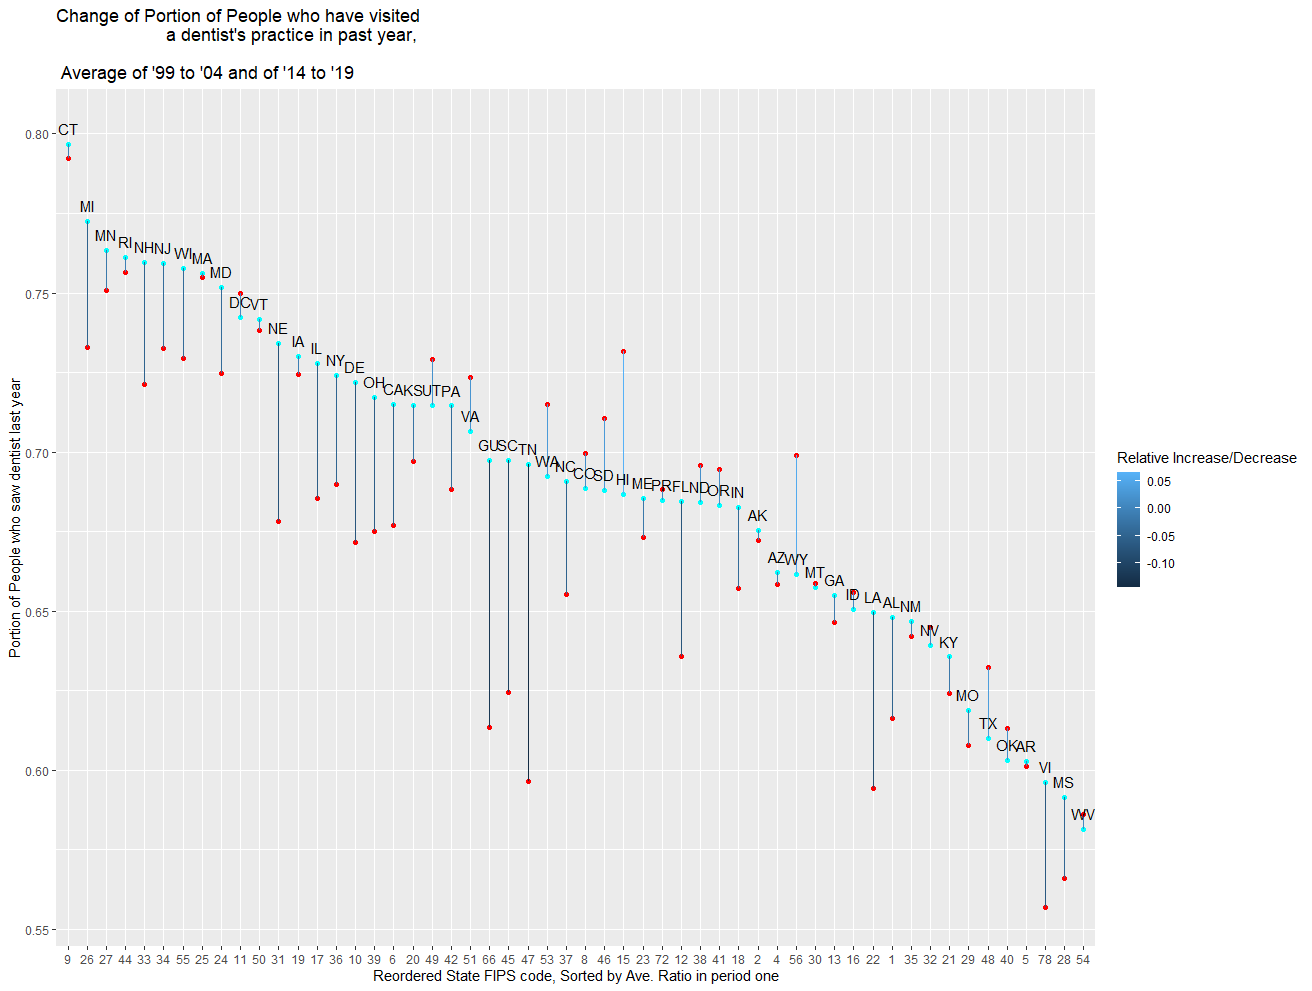
\includegraphics{Change_By_State_02.png}
\caption{Example Graphic One}
\end{figure}

Var\_Name\_1 would be shown as Y-coordiante of cyan dots. Var\_Name\_2
would be shown as Y-coordinate of red dots. The X-coordinates would
matter little and is just FIPS code by state re-ordered by decreasing
order of Var\_Name\_1. Title\_Name gives the upper title.
Change\_Var\_Name is at the left by Y-axis. label\_size refers to the
size of labels indicating which state the data point belongs to, the
two-letter abbreviation near cyan points in the graphic above.

Technical detals and description for each function are in the comments.

\begin{Shaded}
\begin{Highlighting}[]
\NormalTok{State\_Change\_Plotter }\OtherTok{=} \ControlFlowTok{function}\NormalTok{(Input\_Data, Change\_Var\_Name,}
\NormalTok{                                Var\_Name\_1,}
\NormalTok{                                Var\_Name\_2, State\_Var\_Name,}
\NormalTok{                                Title\_Name, }\AttributeTok{label\_size =} \DecValTok{5}\NormalTok{,}
                                \AttributeTok{label\_x\_shift =} \DecValTok{0}\NormalTok{,}
                                \AttributeTok{label\_y\_shift =} \SpecialCharTok{{-}}\NormalTok{.}\DecValTok{015}\NormalTok{)\{}
  
\NormalTok{  Input\_Data }\OtherTok{=} \FunctionTok{as.data.frame}\NormalTok{(Input\_Data) }\DocumentationTok{\#\# To prevent problems}

  \ControlFlowTok{if}\NormalTok{(}\SpecialCharTok{!}\NormalTok{(}\StringTok{"Diff\_Ratio"} \SpecialCharTok{\%in\%} \FunctionTok{colnames}\NormalTok{(Input\_Data)))\{}
\NormalTok{    temp}\SpecialCharTok{$}\NormalTok{Diff\_Ratio }\OtherTok{=}\NormalTok{ (temp[, Var\_Name\_2] }\SpecialCharTok{{-}}\NormalTok{ temp[, Var\_Name\_1]) }\SpecialCharTok{/}
\NormalTok{      temp[, Var\_Name\_1]}
    \DocumentationTok{\#\#\# Find the ratio of difference between two variables to be plotted}
    \DocumentationTok{\#\#\# And compared, if not already done earlier.}
\NormalTok{  \}}
  \ControlFlowTok{if}\NormalTok{(}\SpecialCharTok{!}\NormalTok{(}\StringTok{"State\_FIPS\_Code"} \SpecialCharTok{\%in\%} \FunctionTok{colnames}\NormalTok{(Input\_Data)))\{}
\NormalTok{    temp}\SpecialCharTok{$}\NormalTok{State\_FIPS\_Code }\OtherTok{=} \FunctionTok{fips}\NormalTok{(Input\_Data[, State\_Var\_Name],}
                                \AttributeTok{to =} \StringTok{"fips"}\NormalTok{)}
    \DocumentationTok{\#\#\# Find the FIPS code if not done already.}
\NormalTok{  \}}
  
  \FunctionTok{ggplot}\NormalTok{(}\AttributeTok{data =}\NormalTok{ Input\_Data,}
       \FunctionTok{aes}\NormalTok{(}\AttributeTok{x =} \FunctionTok{reorder}\NormalTok{(State\_FIPS\_Code, }\SpecialCharTok{{-}}\FunctionTok{get}\NormalTok{(Var\_Name\_1))) ) }\SpecialCharTok{+}
  \DocumentationTok{\#\# The base of the plot.}
  \DocumentationTok{\#\# the reorder plot shall re{-}order State\_FIPS\_Code value at Decreasing}
  \DocumentationTok{\#\# order of the values in Var\_Name\_1. The get() function was used}
  \DocumentationTok{\#\# because Var\_Name began as a string and cannot be read directly }
  \DocumentationTok{\#\# by aes.}
    
  \FunctionTok{geom\_point}\NormalTok{(}\FunctionTok{aes\_string}\NormalTok{(}\AttributeTok{y =}\NormalTok{ Var\_Name\_1), }\AttributeTok{col =} \StringTok{"cyan"}\NormalTok{) }\SpecialCharTok{+}
    \DocumentationTok{\#\#\# Get the Y{-}coordinate of some of the scatterplot.}
    \DocumentationTok{\#\# Namely, the ones represented by Var\_Name\_1, colorded Cyan.}
    \DocumentationTok{\#\# Here, there were no get() function because we are using}
    \DocumentationTok{\#\# aes\_string, which can have string input for its parameters,}
    \DocumentationTok{\#\# should such string refers to one of the variable names.}
    
    
  \FunctionTok{geom\_point}\NormalTok{(}\FunctionTok{aes\_string}\NormalTok{(}\AttributeTok{y =}\NormalTok{ Var\_Name\_2), }\AttributeTok{col =} \StringTok{"red"}\NormalTok{) }\SpecialCharTok{+}
    \DocumentationTok{\#\# Another point, for values in Var\_Name\_2}
    \DocumentationTok{\#\# The X{-}coordinate were not defined here so should just inherit from}
    \DocumentationTok{\#\# the first ggplot function.}
    
  \FunctionTok{labs}\NormalTok{(}\AttributeTok{y =}\NormalTok{ Change\_Var\_Name,}
       \AttributeTok{x =} \StringTok{"Reordered State FIPS code, Sorted by Ave. Ratio in period one"}\NormalTok{,}
       \AttributeTok{color =} \StringTok{"Inc/Dec"}\NormalTok{) }\SpecialCharTok{+}
    \DocumentationTok{\#\#\# X and Y axis name, and label for the color of the segment.}
    
  \FunctionTok{geom\_segment}\NormalTok{(}\FunctionTok{aes}\NormalTok{(}\AttributeTok{x =} \FunctionTok{reorder}\NormalTok{(State\_FIPS\_Code, }\SpecialCharTok{{-}}\FunctionTok{get}\NormalTok{(Var\_Name\_1)), }
                     \AttributeTok{xend =} \FunctionTok{reorder}\NormalTok{(State\_FIPS\_Code, }\SpecialCharTok{{-}}\FunctionTok{get}\NormalTok{(Var\_Name\_1)),}
                     \AttributeTok{y =} \FunctionTok{get}\NormalTok{(Var\_Name\_1), }\AttributeTok{yend =} \FunctionTok{get}\NormalTok{(Var\_Name\_2),}
                     \AttributeTok{col =}\NormalTok{ Diff\_Ratio)) }\SpecialCharTok{+}
    \DocumentationTok{\#\#\# Okay so here we have the segmented plot.}
    \DocumentationTok{\#\#\# The segement connects (x,y) and (xend, yend)}
    \DocumentationTok{\#\#\# X{-}coordinate just inherit from previously, using same formula.}
    \DocumentationTok{\#\#\# X{-}end should be same as x, as written above.}
    \DocumentationTok{\#\#\# y{-}coordinates and yend should be values of Var\_Name\_1}
    \DocumentationTok{\#\#\# and Var\_Name\_2 respectively. Those are also coordinates}
    \DocumentationTok{\#\#\# of the two plots we made earlier.}
    \DocumentationTok{\#\#\# The color depends on diff\_ratio.}
    
  \FunctionTok{geom\_text}\NormalTok{(}\AttributeTok{label =}\NormalTok{ Input\_Data[, State\_Var\_Name], }
            \FunctionTok{aes}\NormalTok{(}\AttributeTok{x =} \FunctionTok{reorder}\NormalTok{(State\_FIPS\_Code, }\SpecialCharTok{{-}}\FunctionTok{get}\NormalTok{(Var\_Name\_1)), }
                            \AttributeTok{y =} \FunctionTok{get}\NormalTok{(Var\_Name\_1)),}
            \AttributeTok{nudge\_x =}\NormalTok{ label\_x\_shift, }
            \AttributeTok{nudge\_y =}\NormalTok{ label\_y\_shift,}
            \AttributeTok{size =}\NormalTok{ label\_size) }\SpecialCharTok{+}
    \DocumentationTok{\#\#\# Label the text with coordinates for points showing values of Var\_Name\_1}
    \DocumentationTok{\#\#\# nudge the label as given in input}
    \DocumentationTok{\#\#\# label shall be the state\_var\_name}
    
  \FunctionTok{ggtitle}\NormalTok{(Title\_Name)}
  \DocumentationTok{\#\#\# Add the title}
\NormalTok{\}}
\end{Highlighting}
\end{Shaded}

\hypertarget{examples-for-bls-data.}{%
\subsection{Examples for BLS Data.}\label{examples-for-bls-data.}}

There are several examples. The following chart use BLS Data to picture
the change of dental hygienist per 1,000 people from averages of '99 to
'04 to average of '14 to '19. Technical details are written below

\begin{Shaded}
\begin{Highlighting}[]
\NormalTok{BLS\_Data\_General\_For\_Plotting }\OtherTok{=} 
\NormalTok{  BLS\_Data\_General[BLS\_Data\_General}\SpecialCharTok{$}\NormalTok{occ\_code }\SpecialCharTok{==} \DecValTok{2021}\NormalTok{, ]}
\DocumentationTok{\#\#\# 29{-}2021 is the BLS code for dental hygienists.}
\DocumentationTok{\#\#\# This includes only dental hygienist in the dataset}

\NormalTok{BLS\_Data\_General\_For\_Plotting}\SpecialCharTok{$}\NormalTok{Dtl\_Hyg\_per\_1K\_Pop }\OtherTok{=} 
\NormalTok{  BLS\_Data\_General\_For\_Plotting}\SpecialCharTok{$}\NormalTok{tot\_employment }\SpecialCharTok{/}
\NormalTok{  BLS\_Data\_General\_For\_Plotting}\SpecialCharTok{$}\NormalTok{Est\_Population }\SpecialCharTok{*} \DecValTok{1000}
\DocumentationTok{\#\#\# Find the dental hygienist per 1,000 people data, for each state{-}year}
\DocumentationTok{\#\#\# Named as Dtl\_Hyg\_per\_1K\_Pop}

\NormalTok{BLS\_Data\_General\_For\_Plotting }\OtherTok{=} 
  \FunctionTok{By\_Year\_Operation}\NormalTok{(}\AttributeTok{Input\_Data =}\NormalTok{ BLS\_Data\_General\_For\_Plotting,}
                       \AttributeTok{Var\_Name =} \StringTok{"Dtl\_Hyg\_per\_1K\_Pop"}\NormalTok{,}
                       \AttributeTok{Year\_Var\_Name =} \StringTok{"year"}\NormalTok{,}
                       \AttributeTok{State\_Var\_Name =} \StringTok{"st"}\NormalTok{)}
\DocumentationTok{\#\#\# Process the data and find averages over two period}
\DocumentationTok{\#\#\# of variable Dtl\_Hyg\_per\_1K\_Pop.}
\DocumentationTok{\#\#\# Used default 1999 to 2004 average and 2014 to 2019 average.}

\FunctionTok{State\_Change\_Plotter}\NormalTok{(}\AttributeTok{Input\_Data =}\NormalTok{ BLS\_Data\_General\_For\_Plotting,}
                     \AttributeTok{Change\_Var\_Name =} \StringTok{"Dental Hygienist per 1,000 people"}\NormalTok{,}
                     \AttributeTok{Var\_Name\_1 =} \StringTok{"Dtl\_Hyg\_per\_1K\_Pop\_Average\_1999\_2004"}\NormalTok{,}
                     \AttributeTok{Var\_Name\_2 =} \StringTok{"Dtl\_Hyg\_per\_1K\_Pop\_Average\_2014\_2019"}\NormalTok{,}
                     \AttributeTok{State\_Var\_Name =} \StringTok{"st"}\NormalTok{, }
                     \AttributeTok{Title\_Name =} \StringTok{"Dental Hygienist per 1,000 people }\SpecialCharTok{\textbackslash{}n}
\StringTok{                     Change in 5{-}year average"}\NormalTok{,}
                     \AttributeTok{label\_size =} \DecValTok{2}\NormalTok{)}
\end{Highlighting}
\end{Shaded}

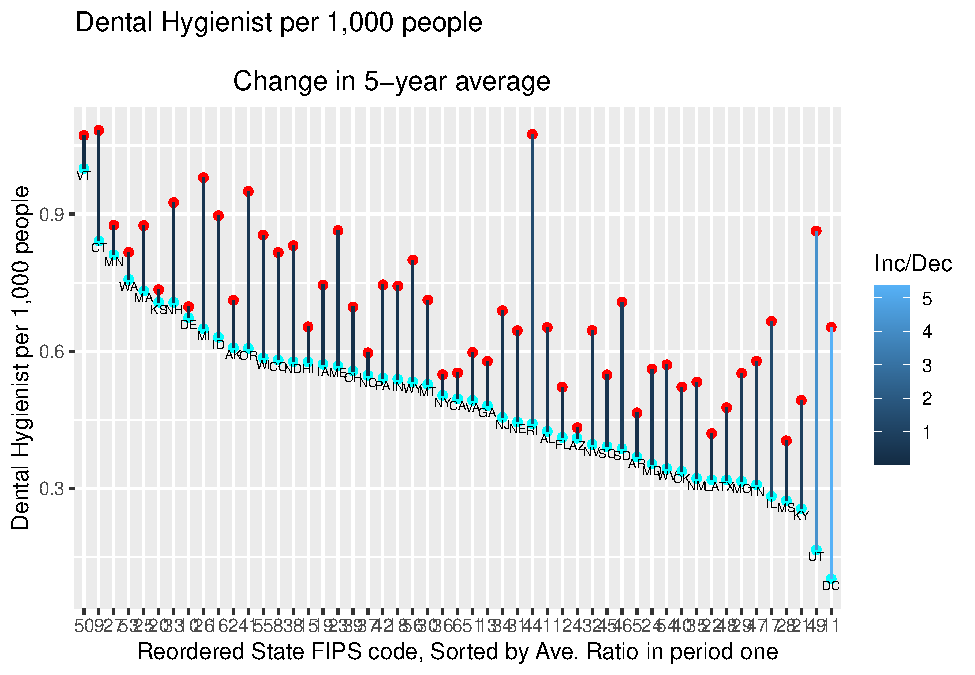
\includegraphics{Change_By_State_Graphic_Reproduction_files/figure-latex/unnamed-chunk-6-1.pdf}

\begin{Shaded}
\begin{Highlighting}[]
\DocumentationTok{\#\#\# Plotting, with self{-}designated title, Y{-}label, etc.}
\end{Highlighting}
\end{Shaded}

We also have a graphic for averaged annual income of dentists (all
dentists, including surgeons etc. Averages were weighed by employment.)
The two periods of average is still 1999 to 2004 and 2014 to 2019.

\begin{Shaded}
\begin{Highlighting}[]
\NormalTok{BLS\_Data\_General\_For\_Plotting }\OtherTok{=} 
\NormalTok{  BLS\_Data\_General[BLS\_Data\_General}\SpecialCharTok{$}\NormalTok{occ\_code }\SpecialCharTok{==} \DecValTok{1020}\NormalTok{, ]}


\NormalTok{BLS\_Data\_General\_For\_Plotting }\OtherTok{=} 
  \FunctionTok{By\_Year\_Operation}\NormalTok{(}\AttributeTok{Input\_Data =}\NormalTok{ BLS\_Data\_General\_For\_Plotting,}
                       \AttributeTok{Var\_Name =} \StringTok{"annual\_mean\_income"}\NormalTok{,}
                       \AttributeTok{Year\_Var\_Name =} \StringTok{"year"}\NormalTok{,}
                       \AttributeTok{State\_Var\_Name =} \StringTok{"st"}\NormalTok{)}

\FunctionTok{State\_Change\_Plotter}\NormalTok{(}\AttributeTok{Input\_Data =}\NormalTok{ BLS\_Data\_General\_For\_Plotting,}
                     \AttributeTok{Change\_Var\_Name =} \StringTok{"Average Annual Income of Dentists"}\NormalTok{,}
                     \AttributeTok{Var\_Name\_1 =} \FunctionTok{colnames}\NormalTok{(BLS\_Data\_General\_For\_Plotting)[}\DecValTok{2}\NormalTok{],}
                     \AttributeTok{Var\_Name\_2 =} \FunctionTok{colnames}\NormalTok{(BLS\_Data\_General\_For\_Plotting)[}\DecValTok{3}\NormalTok{],}
                     \AttributeTok{State\_Var\_Name =} \StringTok{"st"}\NormalTok{, }
                     \AttributeTok{Title\_Name =} \StringTok{"Average Annual Income of Dentists }\SpecialCharTok{\textbackslash{}n}
\StringTok{                     Change in 5{-}year average"}\NormalTok{,}
                     \AttributeTok{label\_size =} \DecValTok{2}\NormalTok{,}
                     \AttributeTok{label\_y\_shift =} \SpecialCharTok{{-}}\DecValTok{1600}\NormalTok{)}
\end{Highlighting}
\end{Shaded}

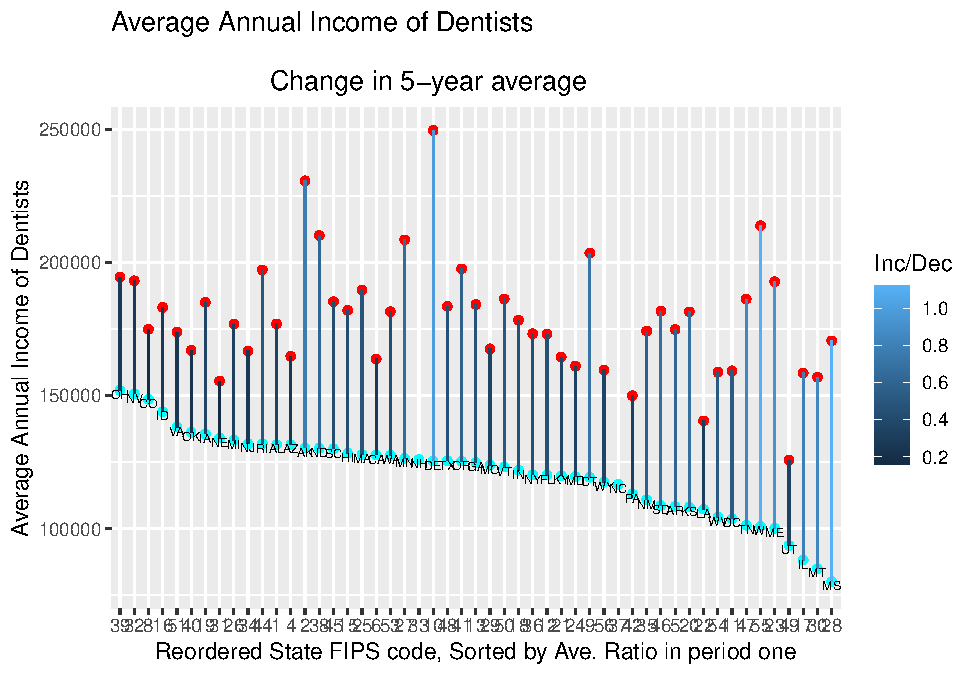
\includegraphics{Change_By_State_Graphic_Reproduction_files/figure-latex/unnamed-chunk-7-1.pdf}

\begin{Shaded}
\begin{Highlighting}[]
\DocumentationTok{\#\#\# Here, since the value is usually some 100,000 to 200,000}
\DocumentationTok{\#\# shifting down 1,600 is not bad}
\end{Highlighting}
\end{Shaded}

\hypertarget{example-brfss-data}{%
\subsection{Example: BRFSS Data}\label{example-brfss-data}}

Firstly, we replicate the graphic we used at foremost as an example,
which is for the portion of people who have not a single teeth removed,
with averages from '99 to '04 and '14 to '19.

\begin{Shaded}
\begin{Highlighting}[]
\NormalTok{BRFSS\_Example\_1 }\OtherTok{=} \FunctionTok{Data\_Condensor}\NormalTok{(}
  \AttributeTok{Input\_Data =}\NormalTok{ Data, }\AttributeTok{Var1 =} \StringTok{"NO\_TEETH\_RMVD"}\NormalTok{, }
  \AttributeTok{Var1\_Condition =} \DecValTok{8}\NormalTok{, }\AttributeTok{Rename\_Columns =} \ConstantTok{TRUE}\NormalTok{)}

\NormalTok{BRFSS\_Example\_1}\SpecialCharTok{$}\NormalTok{st }\OtherTok{=} \FunctionTok{fips}\NormalTok{(BRFSS\_Example\_1}\SpecialCharTok{$}\NormalTok{STATE\_FIPS\_CODE, }\AttributeTok{to =} \StringTok{"abbreviation"}\NormalTok{)}

\NormalTok{BRFSS\_Example\_1 }\OtherTok{=} \FunctionTok{By\_Year\_Operation}\NormalTok{(}\AttributeTok{Input\_Data =}\NormalTok{ BRFSS\_Example\_1,}
                       \AttributeTok{Var\_Name =} \StringTok{"NO\_TEETH\_RMVD\_Ratio"}\NormalTok{,}
                       \AttributeTok{Year\_Var\_Name =} \StringTok{"YEAR\_RESPONSE"}\NormalTok{,}
                       \AttributeTok{State\_Var\_Name =} \StringTok{"st"}\NormalTok{)}

\FunctionTok{State\_Change\_Plotter}\NormalTok{(}\AttributeTok{Input\_Data =}\NormalTok{ BRFSS\_Example\_1,}
                     \AttributeTok{Change\_Var\_Name =} \StringTok{"Portion of People with Not tooth removed"}\NormalTok{,}
                     \AttributeTok{Var\_Name\_1 =} \FunctionTok{colnames}\NormalTok{(BRFSS\_Example\_1)[}\DecValTok{2}\NormalTok{],}
                     \AttributeTok{Var\_Name\_2 =} \FunctionTok{colnames}\NormalTok{(BRFSS\_Example\_1)[}\DecValTok{3}\NormalTok{],}
                      \AttributeTok{Title\_Name =} \StringTok{"Change of Portion of People with not a single tooth removed, }
\StringTok{                     }\SpecialCharTok{\textbackslash{}n}\StringTok{ Average of \textquotesingle{}99 to \textquotesingle{}04 and of \textquotesingle{}14 to \textquotesingle{}19"}\NormalTok{,}
                     \AttributeTok{State\_Var\_Name =} \StringTok{"st"}\NormalTok{, }\AttributeTok{label\_size =} \DecValTok{2}\NormalTok{)}
\end{Highlighting}
\end{Shaded}

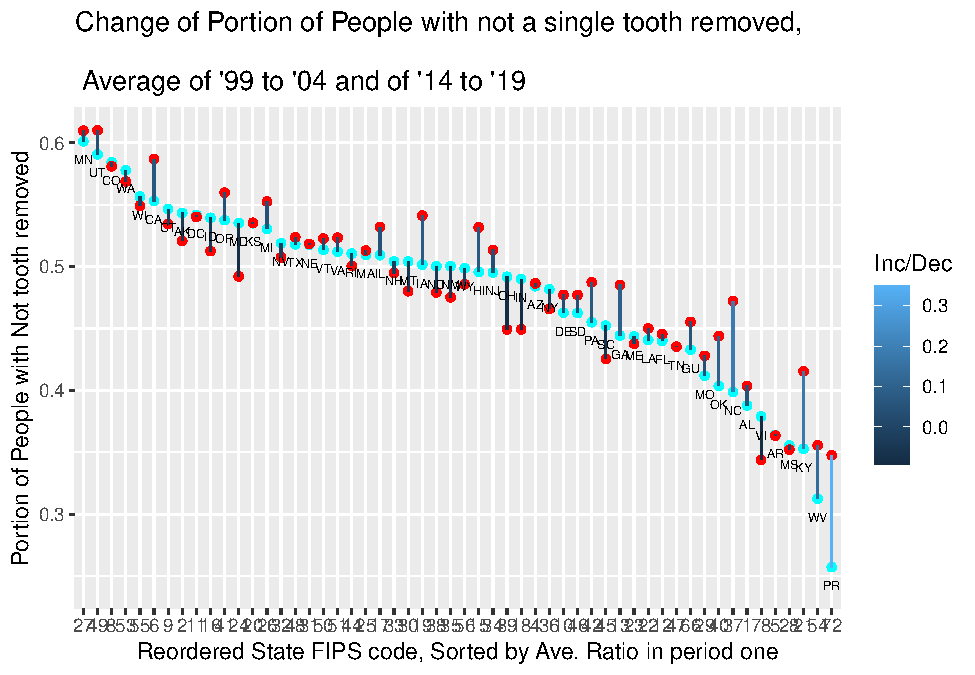
\includegraphics{Change_By_State_Graphic_Reproduction_files/figure-latex/unnamed-chunk-8-1.pdf}

Secondly, we replicate the graphic we used in previous ``Function for
Plotting'' as an example, which is for the portion of people who have
visited a dentist's practice, with averages from '99 to '04 and '14 to
'19.

\begin{Shaded}
\begin{Highlighting}[]
\NormalTok{BRFSS\_Example\_1 }\OtherTok{=} \FunctionTok{Data\_Condensor}\NormalTok{(}
  \AttributeTok{Input\_Data =}\NormalTok{ Data, }\AttributeTok{Var1 =} \StringTok{"DENTIST\_VISIT\_LAST"}\NormalTok{, }
  \AttributeTok{Var1\_Condition =} \DecValTok{1}\NormalTok{, }\AttributeTok{Rename\_Columns =} \ConstantTok{TRUE}\NormalTok{)}

\NormalTok{BRFSS\_Example\_1}\SpecialCharTok{$}\NormalTok{st }\OtherTok{=} \FunctionTok{fips}\NormalTok{(BRFSS\_Example\_1}\SpecialCharTok{$}\NormalTok{STATE\_FIPS\_CODE, }\AttributeTok{to =} \StringTok{"abbreviation"}\NormalTok{)}

\NormalTok{BRFSS\_Example\_1 }\OtherTok{=} \FunctionTok{By\_Year\_Operation}\NormalTok{(}\AttributeTok{Input\_Data =}\NormalTok{ BRFSS\_Example\_1,}
                       \AttributeTok{Var\_Name =} \StringTok{"DENTIST\_VISIT\_LAST\_Ratio"}\NormalTok{,}
                       \AttributeTok{Year\_Var\_Name =} \StringTok{"YEAR\_RESPONSE"}\NormalTok{,}
                       \AttributeTok{State\_Var\_Name =} \StringTok{"st"}\NormalTok{)}

\FunctionTok{State\_Change\_Plotter}\NormalTok{(}\AttributeTok{Input\_Data =}\NormalTok{ BRFSS\_Example\_1,}
                     \AttributeTok{Change\_Var\_Name =} \StringTok{"Portion of People who saw dentist last year"}\NormalTok{,}
                     \AttributeTok{Var\_Name\_1 =} \FunctionTok{colnames}\NormalTok{(BRFSS\_Example\_1)[}\DecValTok{2}\NormalTok{],}
                     \AttributeTok{Var\_Name\_2 =} \FunctionTok{colnames}\NormalTok{(BRFSS\_Example\_1)[}\DecValTok{3}\NormalTok{],}
                      \AttributeTok{Title\_Name =} \StringTok{"Change of Portion of People who have visited }
\StringTok{                      a dentist\textquotesingle{}s practice in past year, }
\StringTok{                     }\SpecialCharTok{\textbackslash{}n}\StringTok{ Average of \textquotesingle{}99 to \textquotesingle{}04 and of \textquotesingle{}14 to \textquotesingle{}19"}\NormalTok{,}
                     \AttributeTok{State\_Var\_Name =} \StringTok{"st"}\NormalTok{, }\AttributeTok{label\_size =} \DecValTok{2}\NormalTok{)}
\end{Highlighting}
\end{Shaded}

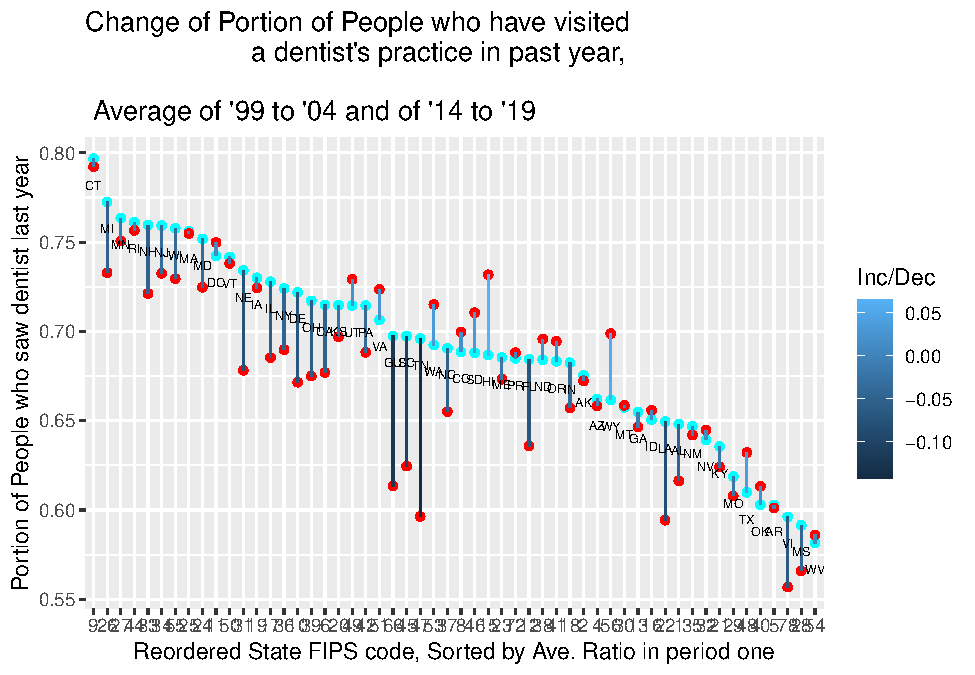
\includegraphics{Change_By_State_Graphic_Reproduction_files/figure-latex/unnamed-chunk-9-1.pdf}

Finally, we produce a graph for the portion of people who have medical
insurance coverage, with averages from '99 to '04 and '14 to '19.

\begin{Shaded}
\begin{Highlighting}[]
\NormalTok{BRFSS\_Example\_1 }\OtherTok{=} \FunctionTok{Data\_Condensor}\NormalTok{(}
  \AttributeTok{Input\_Data =}\NormalTok{ Data, }\AttributeTok{Var1 =} \StringTok{"HEALTH\_PLAN\_STATUS"}\NormalTok{, }
  \AttributeTok{Var1\_Condition =} \DecValTok{1}\NormalTok{, }\AttributeTok{Rename\_Columns =} \ConstantTok{TRUE}\NormalTok{)}

\NormalTok{BRFSS\_Example\_1}\SpecialCharTok{$}\NormalTok{st }\OtherTok{=} \FunctionTok{fips}\NormalTok{(BRFSS\_Example\_1}\SpecialCharTok{$}\NormalTok{STATE\_FIPS\_CODE, }\AttributeTok{to =} \StringTok{"abbreviation"}\NormalTok{)}

\NormalTok{BRFSS\_Example\_1 }\OtherTok{=} \FunctionTok{By\_Year\_Operation}\NormalTok{(}\AttributeTok{Input\_Data =}\NormalTok{ BRFSS\_Example\_1,}
                       \AttributeTok{Var\_Name =} \StringTok{"HEALTH\_PLAN\_STATUS\_Ratio"}\NormalTok{,}
                       \AttributeTok{Year\_Var\_Name =} \StringTok{"YEAR\_RESPONSE"}\NormalTok{,}
                       \AttributeTok{State\_Var\_Name =} \StringTok{"st"}\NormalTok{)}

\FunctionTok{State\_Change\_Plotter}\NormalTok{(}\AttributeTok{Input\_Data =}\NormalTok{ BRFSS\_Example\_1,}
                     \AttributeTok{Change\_Var\_Name =} \StringTok{"Portion of People with Health Plan"}\NormalTok{,}
                     \AttributeTok{Var\_Name\_1 =} \FunctionTok{colnames}\NormalTok{(BRFSS\_Example\_1)[}\DecValTok{2}\NormalTok{],}
                     \AttributeTok{Var\_Name\_2 =} \FunctionTok{colnames}\NormalTok{(BRFSS\_Example\_1)[}\DecValTok{3}\NormalTok{],}
                     \AttributeTok{Title\_Name =} \StringTok{"Change of Portion of People with health plan, }
\StringTok{                     }\SpecialCharTok{\textbackslash{}n}\StringTok{ Average of \textquotesingle{}99 to \textquotesingle{}04 and of \textquotesingle{}14 to \textquotesingle{}19"}\NormalTok{,}
                     \AttributeTok{State\_Var\_Name =} \StringTok{"st"}\NormalTok{, }\AttributeTok{label\_size =} \DecValTok{2}\NormalTok{)}
\end{Highlighting}
\end{Shaded}

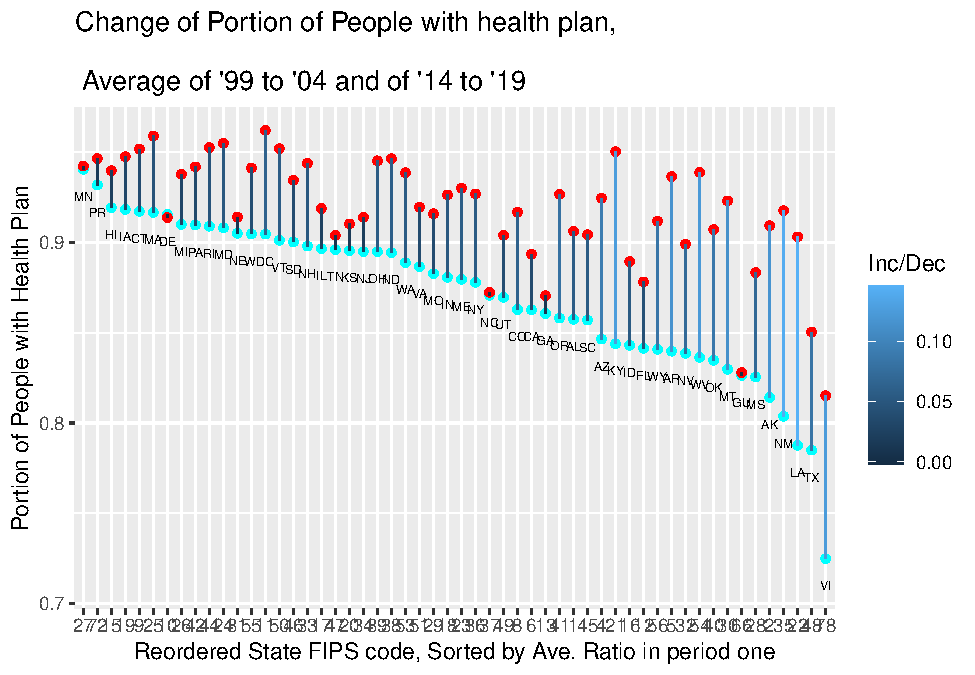
\includegraphics{Change_By_State_Graphic_Reproduction_files/figure-latex/unnamed-chunk-10-1.pdf}

\hypertarget{scatterplot-comparison}{%
\subsection{Scatterplot Comparison}\label{scatterplot-comparison}}

It is also possible to compare two variables of BLS, side-by-side.
Namely, there will two graphics, each showing a scatterplot of two
variables, placed side by side. It was created so that some changes
could be seen relatively easily. The data processing part can be handled
relatively easily with our previous functions, but it still requires
some additional code to do the plotting.

As an example, we will use BLS Data with dental hygienist and dentist
per 1,000 people in two periods.

\begin{Shaded}
\begin{Highlighting}[]
\NormalTok{BLS\_temp\_1 }\OtherTok{=}\NormalTok{ BLS\_Data\_General[BLS\_Data\_General}\SpecialCharTok{$}\NormalTok{occ\_code }\SpecialCharTok{==} \DecValTok{1020}\NormalTok{, ]}

\NormalTok{BLS\_temp\_1}\SpecialCharTok{$}\NormalTok{Dentist\_per\_1K\_Pop }\OtherTok{=} 
\NormalTok{  BLS\_temp\_1}\SpecialCharTok{$}\NormalTok{tot\_employment }\SpecialCharTok{/}\NormalTok{ BLS\_temp\_1}\SpecialCharTok{$}\NormalTok{Est\_Population }\SpecialCharTok{*} \DecValTok{1000}
\DocumentationTok{\#\#\# Find the dentist per 1,000 people data, for each state{-}year}
\DocumentationTok{\#\#\# Named as Dentist\_per\_1K\_Pop}

\NormalTok{BLS\_temp\_1 }\OtherTok{=} 
  \FunctionTok{By\_Year\_Operation}\NormalTok{(}\AttributeTok{Input\_Data =}\NormalTok{ BLS\_temp\_1,}
                       \AttributeTok{Var\_Name =} \StringTok{"Dentist\_per\_1K\_Pop"}\NormalTok{,}
                       \AttributeTok{Year\_Var\_Name =} \StringTok{"year"}\NormalTok{,}
                       \AttributeTok{State\_Var\_Name =} \StringTok{"st"}\NormalTok{)}

\NormalTok{BLS\_temp\_2 }\OtherTok{=}\NormalTok{ BLS\_Data\_General[BLS\_Data\_General}\SpecialCharTok{$}\NormalTok{occ\_code }\SpecialCharTok{==} \DecValTok{2021}\NormalTok{, ]}

\NormalTok{BLS\_temp\_2}\SpecialCharTok{$}\NormalTok{Dtl\_Hyg\_per\_1K\_Pop }\OtherTok{=} 
\NormalTok{  BLS\_temp\_2}\SpecialCharTok{$}\NormalTok{tot\_employment }\SpecialCharTok{/}\NormalTok{ BLS\_temp\_2}\SpecialCharTok{$}\NormalTok{Est\_Population }\SpecialCharTok{*} \DecValTok{1000}
\DocumentationTok{\#\#\# Find the dental hygienist per 1,000 people data, for each state{-}year}
\DocumentationTok{\#\#\# Named as Dtl\_Hyg\_per\_1K\_Pop}

\NormalTok{BLS\_temp\_2 }\OtherTok{=} 
  \FunctionTok{By\_Year\_Operation}\NormalTok{(}\AttributeTok{Input\_Data =}\NormalTok{ BLS\_temp\_2,}
                       \AttributeTok{Var\_Name =} \StringTok{"Dtl\_Hyg\_per\_1K\_Pop"}\NormalTok{,}
                       \AttributeTok{Year\_Var\_Name =} \StringTok{"year"}\NormalTok{,}
                       \AttributeTok{State\_Var\_Name =} \StringTok{"st"}\NormalTok{)}

\NormalTok{BLS\_Data\_General\_For\_Plotting }\OtherTok{=} \FunctionTok{left\_join}\NormalTok{(BLS\_temp\_1, BLS\_temp\_2,}
                                          \AttributeTok{by =} \StringTok{"st"}\NormalTok{)}
\end{Highlighting}
\end{Shaded}

It quickly comes to be that the parameters required---labels and titles
and data frams for two functions--appears to be too much. Thus, instead
of a function with over 10 parameters, I decided to use the raw code,
with instructions below on what could be changed easily within the
coding. Since this is actually only two simple ggplot added together,
much could be done with it.

The chunk shows the first (left) part of the graphic to be shown.

\begin{Shaded}
\begin{Highlighting}[]
\DocumentationTok{\#\# Plot them.}
\NormalTok{A }\OtherTok{=} \FunctionTok{ggplot}\NormalTok{(}\AttributeTok{data =}\NormalTok{ BLS\_Data\_General\_For\_Plotting,}
       \FunctionTok{aes}\NormalTok{(}\AttributeTok{x =}\NormalTok{ Dentist\_per\_1K\_Pop\_Average\_1999\_2004, }
           \AttributeTok{y =}\NormalTok{ Dtl\_Hyg\_per\_1K\_Pop\_Average\_1999\_2004)) }\SpecialCharTok{+}
  \DocumentationTok{\#\#\# Here, you can actually change to whatever dataset with two variables}
  \DocumentationTok{\#\#\# Just like any ggplot plot.}
  
  \FunctionTok{geom\_point}\NormalTok{() }\SpecialCharTok{+}
  \DocumentationTok{\#\#\# To plot scatterplot.}
  
  \FunctionTok{labs}\NormalTok{(}\AttributeTok{y =} \StringTok{"Dental Hygienist per Dentist"}\NormalTok{,}
       \AttributeTok{x =} \StringTok{"Number of Dentist per 1,000 people"}\NormalTok{) }\SpecialCharTok{+}
  \DocumentationTok{\#\#\# Add labels for X and Y axis}
  
  \FunctionTok{geom\_text}\NormalTok{(}\AttributeTok{label =}\NormalTok{ BLS\_Data\_General\_For\_Plotting}\SpecialCharTok{$}\NormalTok{st, }
            \FunctionTok{aes}\NormalTok{(}\AttributeTok{x =}\NormalTok{ Dentist\_per\_1K\_Pop\_Average\_1999\_2004, }
                                       \AttributeTok{y =}\NormalTok{ Dtl\_Hyg\_per\_1K\_Pop\_Average\_1999\_2004),}
            \AttributeTok{nudge\_x =} \DecValTok{0}\NormalTok{, }\AttributeTok{nudge\_y =}\NormalTok{ .}\DecValTok{1}\NormalTok{) }\SpecialCharTok{+}
  \DocumentationTok{\#\#\# Add labels to each data point.}
  \DocumentationTok{\#\#\# The label = argument will be shown at places designated by x{-}y coordinates}
  \DocumentationTok{\#\#\# in aes, and the text shown is what was take in label = argument.}
  \DocumentationTok{\#\#\# The label should be a column from the dataset which were used for plotting }
  \DocumentationTok{\#\#\# The X{-}Y coordinates were designated in aes(), using the same as }
  \DocumentationTok{\#\#\# What the plot began with, though you can change it.}
  
  \FunctionTok{xlim}\NormalTok{(}\DecValTok{0}\NormalTok{, .}\DecValTok{6}\NormalTok{) }\SpecialCharTok{+} \FunctionTok{ylim}\NormalTok{(}\DecValTok{0}\NormalTok{, }\FloatTok{1.3}\NormalTok{) }\SpecialCharTok{+}
  \DocumentationTok{\#\#\# It is advised to fix the X and Y limit if }
  \DocumentationTok{\#\#\# you want to have sensible comparison}
  
  \FunctionTok{geom\_smooth}\NormalTok{(}\AttributeTok{method =} \StringTok{"lm"}\NormalTok{) }\SpecialCharTok{+}
  \DocumentationTok{\#\#\# Add a regression line.}
  \FunctionTok{ggtitle}\NormalTok{(}\StringTok{"Dental Hygienist and Dentist per 1,000 people, }\SpecialCharTok{\textbackslash{}n}
\StringTok{          Averaged \textquotesingle{}99 to \textquotesingle{}04"}\NormalTok{)}
\end{Highlighting}
\end{Shaded}

The second part should be mostly the same in terms of technical details.
Like any GGPLot it can be customized. While I used the same dataset and
two different variables, you can use whatever you want.

\begin{Shaded}
\begin{Highlighting}[]
\NormalTok{B }\OtherTok{=} \FunctionTok{ggplot}\NormalTok{(}\AttributeTok{data =}\NormalTok{ BLS\_Data\_General\_For\_Plotting,}
       \FunctionTok{aes}\NormalTok{(}\AttributeTok{x =}\NormalTok{ Dentist\_per\_1K\_Pop\_Average\_2014\_2019, }
           \AttributeTok{y =}\NormalTok{ Dtl\_Hyg\_per\_1K\_Pop\_Average\_2014\_2019)) }\SpecialCharTok{+}
  \FunctionTok{geom\_point}\NormalTok{() }\SpecialCharTok{+}
  \FunctionTok{labs}\NormalTok{(}\AttributeTok{y =} \StringTok{"Dental Hygienist per Dentist"}\NormalTok{,}
       \AttributeTok{x =} \StringTok{"Number of Dentist per 1,000 people"}\NormalTok{) }\SpecialCharTok{+}
  \FunctionTok{geom\_text}\NormalTok{(}\AttributeTok{label =}\NormalTok{ BLS\_Data\_General\_For\_Plotting}\SpecialCharTok{$}\NormalTok{st, }
            \FunctionTok{aes}\NormalTok{(}\AttributeTok{x =}\NormalTok{ Dentist\_per\_1K\_Pop\_Average\_2014\_2019, }
                                       \AttributeTok{y =}\NormalTok{ Dtl\_Hyg\_per\_1K\_Pop\_Average\_2014\_2019),}
            \AttributeTok{nudge\_x =} \DecValTok{0}\NormalTok{, }\AttributeTok{nudge\_y =}\NormalTok{ .}\DecValTok{1}\NormalTok{) }\SpecialCharTok{+}
  \FunctionTok{xlim}\NormalTok{(}\DecValTok{0}\NormalTok{, .}\DecValTok{6}\NormalTok{) }\SpecialCharTok{+} \FunctionTok{ylim}\NormalTok{(}\DecValTok{0}\NormalTok{, }\FloatTok{1.3}\NormalTok{) }\SpecialCharTok{+}
  \FunctionTok{geom\_smooth}\NormalTok{(}\AttributeTok{method =} \StringTok{"lm"}\NormalTok{) }\SpecialCharTok{+}
  \FunctionTok{ggtitle}\NormalTok{(}\StringTok{"Dental Hygienist and Dentist per 1,000 people, }\SpecialCharTok{\textbackslash{}n}
\StringTok{          Averaged \textquotesingle{}14 to \textquotesingle{}19"}\NormalTok{)}

\FunctionTok{grid.arrange}\NormalTok{(A, B, }\AttributeTok{ncol =} \DecValTok{2}\NormalTok{)}
\end{Highlighting}
\end{Shaded}

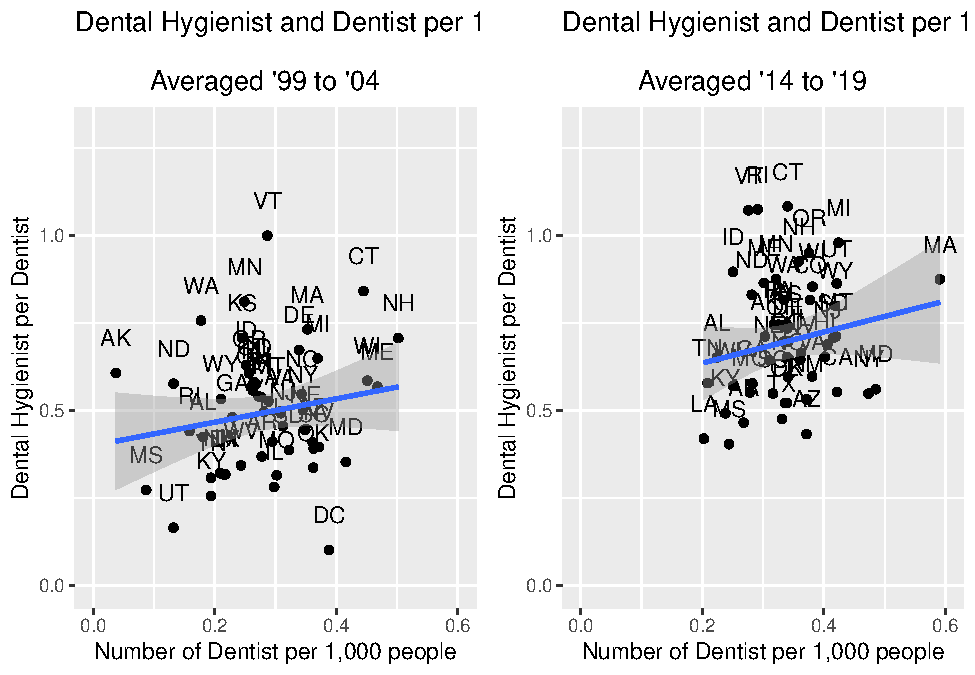
\includegraphics{Change_By_State_Graphic_Reproduction_files/figure-latex/unnamed-chunk-13-1.pdf}

Another example would be finding the correlation of two variables,
dental hygienist per dentist to dentist per 1,000 population. Here is
the plotting used.

The data processing part was hidden because it consisted mainly
primitive techniques and writing them would use up simply too much
space.

And here is the plotting part. Output is BLS\_Merged. Y-axis shows
average dental hygienist to dentist ratio, and X-axis dentist per 1,000
people, averaged.

\begin{Shaded}
\begin{Highlighting}[]
\DocumentationTok{\#\# Plot them.}
\NormalTok{A }\OtherTok{=} \FunctionTok{ggplot}\NormalTok{(}\AttributeTok{data =}\NormalTok{ BLS\_Merged,}
       \FunctionTok{aes}\NormalTok{(}\AttributeTok{x =}\NormalTok{ Dentist\_per\_1K\_Pop\_99\_04, }\AttributeTok{y =}\NormalTok{ Dtl\_Hyg\_per\_Dentist\_99\_04)) }\SpecialCharTok{+}
  \FunctionTok{geom\_point}\NormalTok{() }\SpecialCharTok{+}
  \FunctionTok{labs}\NormalTok{(}\AttributeTok{y =} \StringTok{"Dental Hygienist per Dentist"}\NormalTok{,}
       \AttributeTok{x =} \StringTok{"Number of Dentist per 1,000 people"}\NormalTok{) }\SpecialCharTok{+}
  \FunctionTok{geom\_text}\NormalTok{(}\AttributeTok{label =}\NormalTok{ BLS\_Merged}\SpecialCharTok{$}\NormalTok{st, }\FunctionTok{aes}\NormalTok{(}\AttributeTok{x =}\NormalTok{ Dentist\_per\_1K\_Pop\_99\_04, }
                                       \AttributeTok{y =}\NormalTok{ Dtl\_Hyg\_per\_Dentist\_99\_04),}
            \AttributeTok{nudge\_x =} \DecValTok{0}\NormalTok{, }\AttributeTok{nudge\_y =}\NormalTok{ .}\DecValTok{1}\NormalTok{) }\SpecialCharTok{+}
  \FunctionTok{xlim}\NormalTok{(.}\DecValTok{25}\NormalTok{, }\FloatTok{1.1}\NormalTok{) }\SpecialCharTok{+} \FunctionTok{ylim}\NormalTok{(.}\DecValTok{5}\NormalTok{, }\FloatTok{4.5}\NormalTok{) }\SpecialCharTok{+}
  \FunctionTok{geom\_smooth}\NormalTok{(}\AttributeTok{method =} \StringTok{"lm"}\NormalTok{) }\SpecialCharTok{+}
  \FunctionTok{ggtitle}\NormalTok{(}\StringTok{"Dental Hygienist per Dentist VS Dentist per 1,000 people, \textquotesingle{}99 to \textquotesingle{}04"}\NormalTok{)}

\NormalTok{B }\OtherTok{=} \FunctionTok{ggplot}\NormalTok{(}\AttributeTok{data =}\NormalTok{ BLS\_Merged,}
       \FunctionTok{aes}\NormalTok{(}\AttributeTok{x =}\NormalTok{ Dentist\_per\_1K\_Pop\_14\_19, }\AttributeTok{y =}\NormalTok{ Dtl\_Hyg\_per\_Dentist\_14\_19)) }\SpecialCharTok{+}
  \FunctionTok{geom\_point}\NormalTok{() }\SpecialCharTok{+}
  \FunctionTok{labs}\NormalTok{(}\AttributeTok{y =} \StringTok{"Dental Hygienist per Dentist"}\NormalTok{,}
       \AttributeTok{x =} \StringTok{"Number of Dentist per 1,000 people"}\NormalTok{) }\SpecialCharTok{+}
  \FunctionTok{geom\_text}\NormalTok{(}\AttributeTok{label =}\NormalTok{ BLS\_Merged}\SpecialCharTok{$}\NormalTok{st, }\FunctionTok{aes}\NormalTok{(}\AttributeTok{x =}\NormalTok{ Dentist\_per\_1K\_Pop\_14\_19, }
                                       \AttributeTok{y =}\NormalTok{ Dtl\_Hyg\_per\_Dentist\_14\_19),}
            \AttributeTok{nudge\_x =} \DecValTok{0}\NormalTok{, }\AttributeTok{nudge\_y =}\NormalTok{ .}\DecValTok{1}\NormalTok{) }\SpecialCharTok{+}
  \FunctionTok{xlim}\NormalTok{(.}\DecValTok{25}\NormalTok{, }\FloatTok{1.1}\NormalTok{) }\SpecialCharTok{+} \FunctionTok{ylim}\NormalTok{(.}\DecValTok{5}\NormalTok{, }\FloatTok{4.5}\NormalTok{) }\SpecialCharTok{+}
  \FunctionTok{geom\_smooth}\NormalTok{(}\AttributeTok{method =} \StringTok{"lm"}\NormalTok{) }\SpecialCharTok{+}
  \FunctionTok{ggtitle}\NormalTok{(}\StringTok{"Dental Hygienist per Dentist VS Dentist per 1,000 people, \textquotesingle{}14 to \textquotesingle{}19"}\NormalTok{)}


\FunctionTok{grid.arrange}\NormalTok{(A, B, }\AttributeTok{nrow =} \DecValTok{2}\NormalTok{)}
\end{Highlighting}
\end{Shaded}

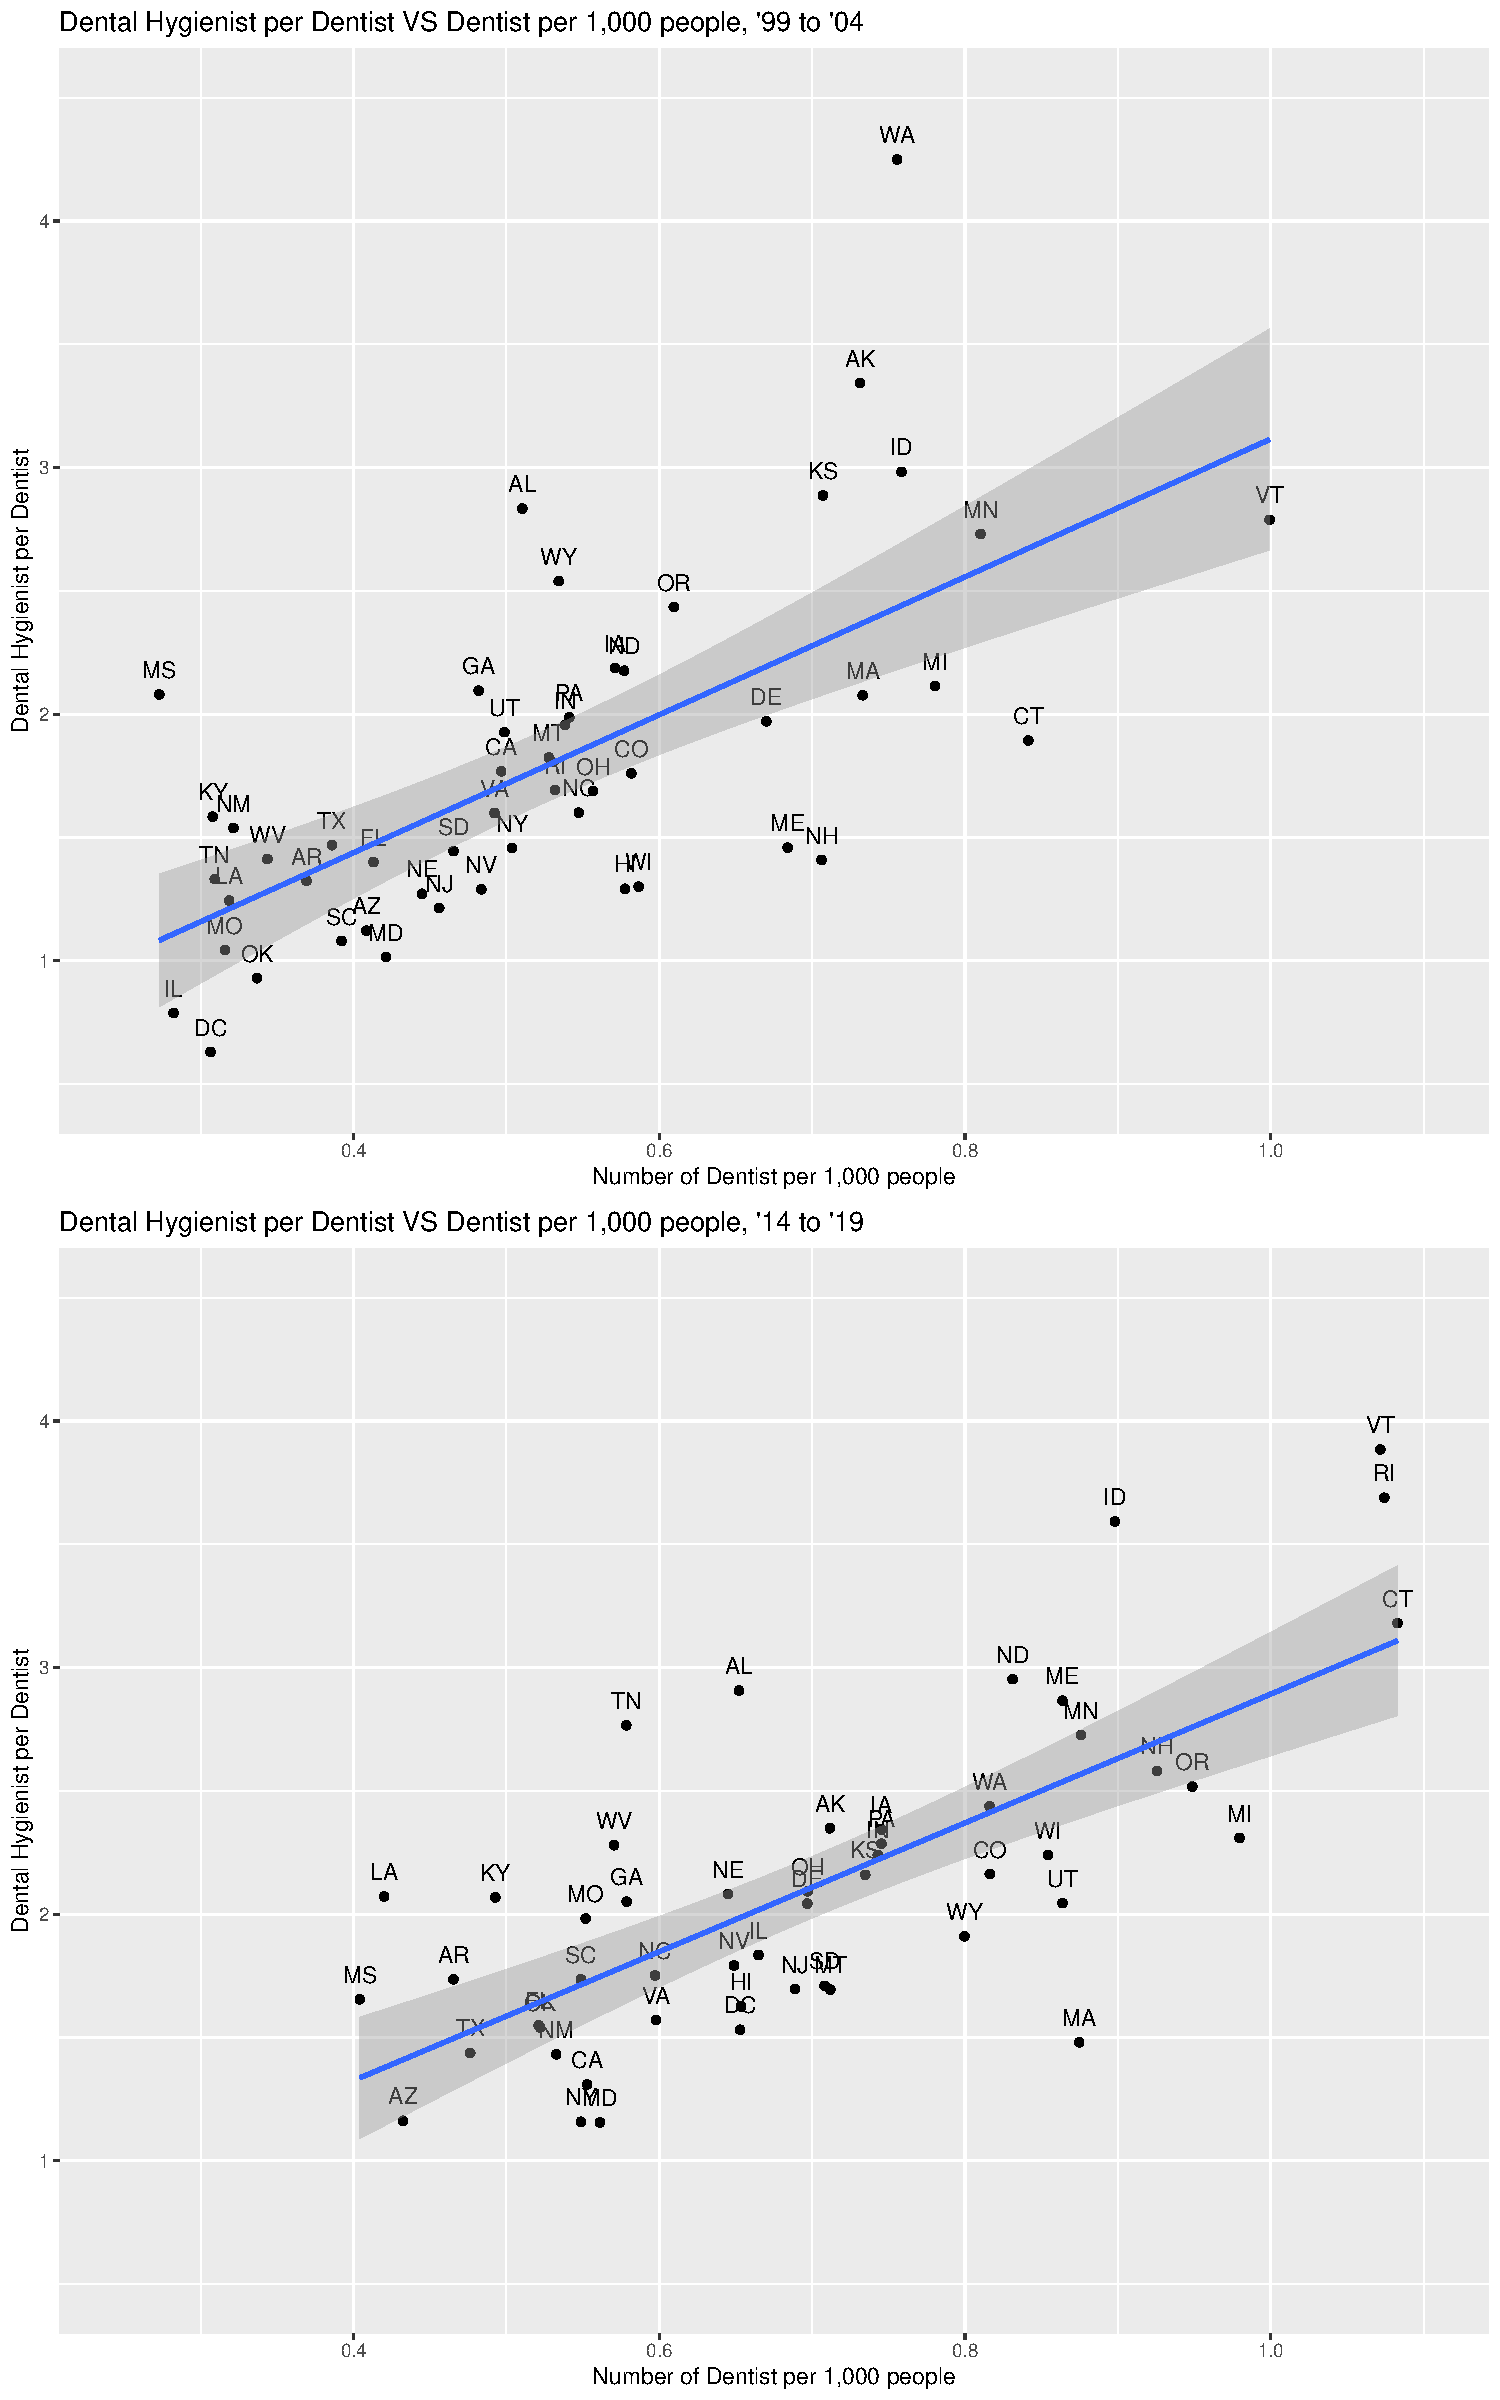
\includegraphics{Change_By_State_Graphic_Reproduction_files/figure-latex/unnamed-chunk-15-1.pdf}

\end{document}
